\documentclass[12pt]{report}
\usepackage[a4paper, total={6in, 9in}]{geometry}
\usepackage{graphicx}
\usepackage{amsmath}
\usepackage{gensymb}
\usepackage{cclicenses}
\usepackage{listings}
\usepackage[framemethod=tikz]{mdframed}
\usepackage{url}
\newcommand{\ignoreoverfullhboxes}{\setlength{\hfuzz}{\maxdimen}}
\bibliographystyle{plain}


\begin{document}
\begin{titlepage}
\begin{center}
\vspace*{1cm}
\huge
\textbf{Development of an Open Source Chemical Process Simulator} \\
\vspace*{0.7cm}
\Large
Submitted in partial fulfillment of the requirements of the degree of Master of Technology \\
\vspace{0.5cm}
\Large
by \\
\vspace{0.4cm}
\LARGE
\textbf{Rahul Jain} \\
(Roll No. 143020028) \\
\vspace{0.8cm}
\LARGE
Supervisor: \\
\textbf{Prof. Kannan . M . Moudgalya} \\
\vspace{1cm}

\includegraphics[width=0.4\textwidth]{university} \\
\vspace{1cm}
\Large
Chemical Engineering Department \\
\vspace{0.5cm}
INDIAN INSTITUTE OF TECHNOLOGY BOMBAY \\
2016
\end{center}
\end{titlepage}

\section*{Approval Sheet}
This thesis entitled $"$Development of an Open Source Chemical Process Simulator$"$ by Rahul Jain (Roll no. 143020028) may be accepted for being evaluated for the award of the degree of Master of Technology. \\
\vspace{1.5cm}
\begin{flushright}
......................... \\
Prof. Kannan Moudgalya (Supervisor) \\
\vspace {1cm}
......................... \\
Prof. V. Dalvi (Examiner) \\
\vspace {1cm}
......................... \\
Prof. Y. Shastri (Examiner) \\
\vspace {1cm}
......................... \\
Prof. D. B. Phatak(Chairperson) \\
\end{flushright}

\newpage

\section*{Declaration}
I, \textbf{Rahul Jain}, Roll No. 143020028, declare that the work presented in this report is carried out by my own. Also, wherever someone else's ideas have been used, they have been cited and nothing has been copied verbatim. Due credit has been given to all the contibutors and authors, whose ideas and theories reflecting in this project report. \\
\vspace{3cm}

\begin{flushright}
........................ \\
Rahul Jain(143020028)
\end{flushright}

\vspace{3cm}

\begin{flushleft}
Date: 06 July 2016
\end{flushleft}

\newpage
\section*{Acknowledgements}
Firstly, I would like to thank my supervisor Prof. Kannan. M. Moudgalya, for guiding me throughout this project. The door to Prof. Moudgalya's office was always open whenever I ran into a trouble spot or had a question about my research. He consistently steered me in the right direction whenever he thought I needed it.

I would also like to thank Prof. K. P. Madhvan for providing me with rich literature sources. His expertise and broad knowledge has been of great value to me.  

I would also like to thank the following interns Mr. Arpit Gupta, Mr. Neelesh Chandran, Mr. Jairam Ganesh and Mr. Rahul Nagraj. Their hard work and innovative ideas has been of great help to me. 


\abstract
Openmodelica is a state of art equation oriented modeling environment capable of doing both steady state and dynamics simulation but lacks thermodynamics, and good chemical engineering support. DWSIM is a sequential modular steady state simulator with good thermodynamic library (DTL). An attempt is made to make DTL available for Openmodelica in this work. Python-C API and Socket programming approaches are implemented and the performance compared for tasks like steady state and transient simulations regarding chemical engineering systems in Openmodelica. Socket programing performs much better in all the attempted examples. But both the approaches failed when it comes to solving complex chemical engineering processes. Therefore an attempt is made to develop an in-built thermodynamic engine in openmodelica so that thermodynamic equations can be solved simultaneously with mass and energy balance. This built in thermodynamic engine proved to be successful in solving many complex processes with excellent speed and accuracy. 
\tableofcontents
\listoftables
\listoffigures

\chapter{Introduction}
A chemical process simulator is a software through which one can perform chemical engineering calculations. As all the calculations are done by a computer, chemical process simulator provides a robust and fast way to carry out the calculations, rather than doing it manually.

Presently many commercial chemical process simulators are available, which can be used for educational and industrial purposes. But as these commercial process simulators are very expensive, only large scale industries and very few academic institutes can a afford it. Aspen plus, Chemcad, Pro II are some of the commercial chemical process simulators presently available in the market. Due to this reason there is a strong need to develop an open source, free chemical process simulator, so that it can be used by small scale industries and academic institutes.

The open source chemical process simulators that are currently available, have some drawbacks, due to which they cannot replace the commercial process simulators. DWSIM is one such steady state process simulator which is open source and has excellent built in thermodynamic and unit operations, but the only drawback is that it is not fit for design and dynamic simulation. Whereas openmodelica is a state of art simulation and modeling environment, which is excellent for design and dynamic simulations but doesn't have a thermodynamic engine and library of unit operations. Therefor if one can successfully develop a thermodynamic engine in openmodelica, it can become an alternate to the commercial chemical process simulators, which is beneficial for both small scale industries and academic institutes. There are two ways of carrying out the above task. 
\begin{itemize}
\item Integrating the thermodynamic engine of DWSIM with openmodelica. In this process the thermodynamic calculations will be performed by DWISIM where as the unit operation modeling equations which are mostly mass and energy balances will be solved by openmodelica solvers. 
\item Developing a new thermodynamic engine from scratch in openmodelica itself. This includes the development of compound database and all the thermodynamic routines and VLE packages required for a powerful thermodynamic engine. In this approach all the thermodynamic equations and the unit operations modelling equations will be solved simultaneously by openmodelica solvers.
\end{itemize}

\chapter{Open Source Chemical Process Simulator}

\section{Chemical Process Simulators}

\subsection{What is it ?}
Chemical Process simulator is a software that can be used to design, optimize, analyze and develop chemical processes.Chemical Process simulation is a model based representation of unit operations in software. Basic prerequisites   are a thorough knowledge of chemical and physical properties of pure components and mixtures, of reactions, and of mathematical models which, in combination, allow the calculation of a process in computer.
Chemical Process simulation software describes processes in flow diagrams where unit operations are positioned and connected by product streams. The software has to solve the mass and energy balance to reach a stable operating point. The goal of a process simulation is to reach optimal conditions for an examined process. This is essentially an optimization problem which has to be solved in an iterative process.
Chemical Process simulation always use models which introduce approximations and assumptions but allow the description of a property over a wide range of temperatures and pressures which might not be covered by real data. Models also allow interpolation and extrapolation within certain limits and enable the search for conditions outside the range of known properties.
A chemical process simulator which is free of cost, with its source available and editable is knows as open source chemical process simulator.

\subsection{Various Components of a Chemical Process Simulator}
\begin{itemize}
\item{\textbf{Component Database}} \\
A component database is a library of all the components and their physical properties. It contains constant and equations for calculation of physical properties at different pressures and temperatures. Some of these physical property constants are Antoin's coefficients, heat capacity, density, heat of formation, critical temperature and pressure. The simulator accesses all the physical property data from this database and hands it over to the solver at run time. Some of the commercially available component databases are DCHEMA and Nist. Chemsep and DWSIM are two open source component database.

\item{\textbf{Thermodynamics}} \\
All chemical process simulator need a library of routines that calculate thermodynamic data such as VLE parameters, dew and bubble point pressures and temps., vapor and liquid enthalpies, viscosities, densities, and other physical and transport properties of pure component and mixtures .Various thermodynamic models have been developed to fulfill this requirement as a single model cannot predict the properties of all the components.All these thermodynamic models are present in thermodynamic engine of a process simulator.It is the thermodynamic engine that decides how robust a simulator is. Choosing the right model is extremely important because using the wrong model, or estimating a physical property incorrectly, can lead to inaccurate results for the overall simulation.

\item{\textbf{Unit Operation Modules}} \\
Every process simulator has a library of unit operation modules which replicates the physical/chemical operation of the actual process unit of the plant like Heat Exchangers, Distillation Columns, Pumps, Computer compressors, etc. These unit operation modules consists of a set of equations which relates thermodynamic behavior of input stream variables to that to the output stream variables. Most of the the unit operation involves highly non-linear algebraic equation which has to solved by
a solver which does it by some numerical iterative method as mostly analytical solution is not possible.

\item{\textbf{Solver}} \\
The solver solves all the equations that are given to it by the thermodynamic engine and all unit modules included in the flowsheet. Depending on the flowsheet there may be two types of processes namely acyclic and recycle. In acyclic calculation order is generally straight forward and is in the direction of material flow. In recycle processes the flow sheet is divided into a number of single or nested recycle loops and the minimum number of tear streams ( can be recycle streams) are identified . The calculation sequence of module is thus determined as a result of this tearing. The solver solves these equations with the help of some numerical iterative method.
\end{itemize}

\subsection{Applications of Chemical Process Simulators in Education and Industry}
\begin{itemize}
\item{\textbf{Helps in learning chemical engineering concepts.}} \\
One can generate various parametric graphs and observe the nature for better understanding of the concepts.

\item{\textbf{Visualization of the whole plant.}} \\
By looking at the flowsheeting section of a simulator one can visualize the mass and energy flow of a plant.

\item{\textbf{Helps in project work.}} \\
Students can use a simulator to perform calculations related to their projects which otherwise would be very time consuming if done manually. All the thermodynamic and transport properties at various temperatures and pressures can also be extracted which are required in most of the project work.

\item{\textbf{Process plant synthesis.}} \\
New process can be checked for feasibility study. Comparative studies can also be performed to decide which process would be more efficient for the production of required compound.

\item{\textbf{Estimation of Parameters.}} \\
Based on the experimental data various parameters can be estimated by the simulator's build in data fitting techniques. For example binary interaction parameters, rate constants of reaction, order of reactions can be predicted.

\item{\textbf{Used for design of unit operations.}} \\
One can come out with an optimized design for unit operations for a given load.

\item{\textbf{Optimization of Operating Parameters.}} \\
Simulators can be used to study the effect of changing various parameters (pressure, temperature, flow rate etc.) on plant efficiency and product purity. This eliminates the need of pilot plants, which were quite cost intensive.

\item{\textbf{Designing control strategies.}} \\
Control strategies can be designed and tested before applying it on the actual plant.

\item{\textbf{Cost estimation.}} \\
Cost estimation can be done which gives an idea whether the process is economically feasible or what will be the revenue generated.

\item{\textbf{Safety.}} \\
All the parametric changes can be done on the simulator instead of applying it directly on the plant which may lead to some hazardous or dangerous situations. Safety systems can also be designed on Simulator.
\end{itemize}

\section{Why an Open Source Chemical Process Simulator}

\subsection{Expensive for academic institutions}
Commercial process simulator are very expensive even for educational purposes. Most of the chemical engineering institutes exclude process simulation course from their curriculum as Commercial simulators are not affordable.

Simulation is a valuable tool to understand the principles of chemical engineering. It will also help simulate large scale, industrial level, problems, which is not possible by paper and pen. A student who is well trained in simulation will be extremely useful to the industry. This will help to improve employment of chemical engineering students.

\subsection{Expensive for Industry}
Commercial process simulators are not affordable for small and medium scale industries. Hiring consulting firms is not an option because presently all consulting firms use commercial simulators and therefore the consulting charges are very high. Therefore most of them are poorly designed, which reduces the efficiency of the plant. Industry can use an open source simulator for resolving their problems or take help from individuals who knows open source simulation.

Small chemical consulting firms can be established which uses open source simulators, to resolve industrial problems.These consulting firms can be started with almost zero investment as they will be using an open source simulator. The consulting charges will also be reasonably low as commercial simulator are not used.

This way both the consulting firms and the manufacturing firms can be mutually helpful to each other.

\subsection{Amenable to the conduct of large scale training.}
As open source simulators are freely available, anyone who is an expert can share his/her expertise without any legal constraints. Following three workshops were conducted by FOSSEE to spread awareness and learning of DWSIM which is an open source process simulator.
\begin{itemize}
\item{Workshop conducted at Azeotropy, IIT Bombay. Participants were only students.}
\item{Workshop conducted by FOSSEE at IIT Bombay. Professors and people from industry also attended.}
\item{Workshop conducted at ICT, Mumbai. Participants were only students.}
\end{itemize}

\chapter{Literature Survey}
\section{Available commercial chemical process simulation environments and their thermodynamic engine}
\subsection{gPROMS ModelBuilder}
gPROMS ModelBuilder is an environment for modelers to build, validate and execute steady-state and dynamic process models based on the gPROMS second-generation EO modeling platform originally developed at Imperial College London [Barton and Pantelides, 1994; Oh and Pantelides,1996], and subsequently substantially re-architected and re-written at PSE. Following are the thermodynamic engines that can be used in gPROMS to perform chemical process simulations. \cite{GP}
\begin{itemize}
\item \textbf{Multiflash thermodynamic engine} \\
KBC Advanced Technologies' Multiflash is the standard gPROMS physical properties package. It is supplied as an integral part of gPROMS Process Builder, along with the 2000+ component DIPPR 801 database.

Multiflash is a highly rigorous properties package that supports all commonly used thermodynamic and transport properties, including a wide range of equation of state and activity coefficient thermodynamic models.

Multiflash is specifically designed for equation-orientated modeling, providing tight convergence of internal iterations and analytical partial derivatives with respect to temperature, pressure and composition.

PSE can supply Multiflash with the DIPPR database supplied by the AIChE, providing component data for thousands of components.

\item \textbf{OLI electrolyte properties} \\
PSE provides OLI Systems' OLI electrolyte properties package for aqueous electrolytic systems. It is a proprietery thermodynamic package and involves separate licensing cost.

\item \textbf{CAPE-OPEN physical properties} \\
gPROMS provides a CAPE-OPEN physical properties socket into which any CAPE-OPEN compliant physical properties package can be plugged – for example Aspentech's Aspen Properties, PROSIM's SIMULIS Thermodynamics, Aspentech's COMThermo and many others.

\item \textbf{gSAFT} \\
Statistical Associating Fluid Theory, or SAFT, is an advanced molecular thermodynamic method that can predict a wide variety of thermodynamic properties of mixtures accurately based on physically-realistic models of molecules and their interactions with other molecules.
\end{itemize}

\subsection{Aspen Custom Modeler}
Aspen-tech' Aspen custom modeler is a modeling and simulation environment to develop customized model. It is an evolution of SPEEDUP, a first-generation EO
tool originally developed at Imperial College London [Pantelides, 1988].

The primary purpose of custom modeler is to built customized process models which are not available in Aspen Plus or Apen Hysys. These models can then be imported to Aspen plus or hysys and can be integrated with the flowsheet. 

The custom modeler attains its thermodynamics from aspen properties which is a proprietery thermodynamic engine developed by Aspen-tech. Aspen properties itself uses two popular databases, namely NIST and DCHEMA.

The thermodynamic equations are calculated separately by aspen properties, whereas the modeling equations are solved separately by aspen custom modeler. \cite{ACM}

\section{Open source simulation environment and associated thermodynamic engine}
\subsection{ASCEND}
ASCEND is also an open source simulation environment based on equation oriented approach. ASCEND has developed its own thermodynamic engine based on the book \'The Properties of Gases and Liquids'\ \cite{ascend} which provides pure component properties for compounds. This thermodynamic engine is named as fprops  \cite{fprops}. The problem with ASCEND thermodynamic is that is has very limited thermodynamic package support for example their is support for only one thermodynamic activity which is UNIQUAC. Another problem is that the compound database is not intensive.



\chapter{DWSIM: An Open Source Steady State Process Simulator}
\section{The Sequential Modular Approach} \cite{SM}
\subsection{What is Sequential Modular Approach}
DWSIM is based on sequential modular approach. In this approach there are computer programs for all unit operations. One constructs a complete model of these units by writing modeling equations, keeping in mind some assumptions, which closely replicates the actual process units. The simulator then solves the total process flowsheet by calling each unit according to how they are connected in the flowsheet and iterating where loops are encountered. In this approach the variables(pressure, temperature, flows, composition) to input streams to the are fixed and it will compute the variables of the streams leaving the unit. Apart from specifying the input streams completely one has to specify the unit parameters as well, for example the flash unit requires one to specify the temperature and pressure at which the flashing takes place. The degree of freedom should be zero. The solver used for solving the equations is developed so efficiently that it takes some default initial guess values to calculate the solution through some numerical iterative technique. These guess values are then updated and progressively the system converges.

\subsection{The Two Pillars of Sequential Modular Approach} \cite{SM}
\begin{itemize}
\item{Partitioning and Precedence Order} \\
The units we have to solve together are called partitions. The entire flowsheet is divided into partitions and then a precedence order is determined which decides which partition should be calculated according to the connectivity of the partitions. The results of each partition depends on its input and the units contained within that partition and not on any other units. The grouping is unique, while the ordering may or may not be, depending on the particular flowsheet under examination
\item{Tearing} \\
The next issue is how we might solve each of the partitions containing more than a single unit, which have a looping structure. Looping occurs when stream passes through different units and returns back to the same unit in a cyclic fashion. To break this loop tearing is done which enforces an acyclic flow.
\end{itemize}

\subsection{Advantages and Disadvantages of Sequential Modular Approach}

\begin{itemize}
\item {The models of the different units can be prepared and tested separately, while the unit model can be expressed as a computer program subroutine(procedure).}
\item{The solution method for a single unit can be optimized.}
\item{Because of rigid requirements, input data can be quite easily checked for completeness and consistency.}
\item{Because of the modular structure, new units are easily added to the flowsheeting program.}
\item{Less attractive strategy when dealing with design and optimization problems.}
\end{itemize}

\section{Good collection of Unit Operations and Flowsheeting Applications}

\subsection{Unit Operations in DWSIM}

DWSIM has a rich library of built in unit operations which covers almost all the major unit operations used in any chemical industry. These unit modules can easily be inserted into the flowsheet by just dragging them to the flowsheet. The units can then be connected to input and output material streams and energy streams if required. The flowsheet can then be simulated to calculate the output stream properties.
Apart from this if one wants to insert a new unit module, DWSIM provides the facility of building your own custom unit operations. For customizing a module DWSIM provides two options.

\begin{itemize}
\item {\textbf{Spread Sheet Unit Operation}} \\
This module uses a spreadsheet application like excel or Libre office calc to model the unit which can then be inserted directly into the flowsheet. The spreadsheet consists of three sheets namely input, output and calculation. The variable in the input and output sheets are predefined by DWSIM and the user must not edit it. The variables in the input sheet automatically takes the values from the input material stream at run time. All the modeling equations must be inserted in the calculation sheet which takes values from input sheet and return calculated values to output sheet.
\item{\textbf{Custom unit Operation}} \\
This module uses a programming language where the user can code the required unit module, after which the module can directly be inserted into the flowsheet. The two programming languages which can be used for this purpose are iron python and visual basic.
\end{itemize}

\subsection{Flowsheeting Applications in DWSIM}
\begin{itemize}
\item {\textbf{Column profiles}} \\
Column profiles are very important as they give idea of how various parameters like temperature, pressure, composition, flows vary along the length of the column. By studying these profiles one can decide various design aspects of the column like number of trays, the optimal feed stage etc. DWSIM can generate column profiles of distillation, absorption and extractive columns.

\item{\textbf{Sensitivity Analysis}} \\
Sensitivity analysis is varying an independent variable over a given range and observing the behavior of dependent variable accordingly. This feature helps optimize parameters. For example the behavior of product composition and reboiler duty can be observed by varying the reflux ratio and the number of trays so that one obtain an optimized value of both. Sensitivity analysis is not confined to only a single unit operation, it can be implemented between any two variables of the entire flowsheet.

\item{\textbf{Multivariable Optimizer}} \\
It is similar to sensitivity analysis but instead of generating a plot it directly gives the optimized value of the parameter. Another advantage of multi variable optimizer is that, here one can define an objective function like cost, efficiency etc. which can be minimized or maximized.

\end{itemize}

\section{Thermodynamics}
\subsection{Thermodynamic packages available in DWSIM}
DWSIM in enriched with strong thermodynamic engine which can extract physical property data from the two available databases namely Chemsep and DWSIM. It can also extract properties from any other databases which is in .xml format. DWSIM has a rich set of thermodynamic packages which includes ideal gas, equation of state, activity coefficient models. This makes it versatile to simulate any kind of system in DWSIM.

\subsection{Flash Algorithm} \cite{DWSIM}
Flash algorithm are thermodynamic procedures which calculates the properties of output streams after the input stream is flashed, for given operation conditions. In principle, flash calculations are straightforward and involve combining the VLE equations with the component mass balances, and in some cases energy balance also. Following are the four flash algorithms one can use in DWSIM according to the process requirement.

\begin{itemize}
\item{\textbf{PT Flash}} \\
This is the simplest flash algorithms. One has to specify pressure and temperature for implementing it. It involves overall and component mass balance, VLE equations and mole fraction summation equations.
\item{\textbf{PH Flash}} \\
This is pressure and enthalpy flash algorithm. It involves overall and component mass balance, VLE equations, mole fraction summation equations and energy balance equation.
\item{\textbf{PV Flash}} \\
This is the pressure and vapor fraction flash algorithm. One needs to specify the pressure and vapor fraction and the algorithm will calculate temperature and composition of the resulting vapor and liquid streams. The dew point and bubble point calculations of any mixture are performed by this flash. For bubble point set the vapor fraction as zero and for dew point set the vapor fraction as one. It involves overall and component mass balance, VLE equations and mole fraction summation equations.
\item{\textbf{PS Flash}} \\
This is the pressure and entropy flash algorithm. It involves the same equations as of PH flash, but the energy balance equation in PH flash is replaced by entropy balance here.
\end{itemize}

\subsection {Thermodynamic Curves and Parameter Estimation}
DWSIM offers the facility to plot various thermodynamic plots like VLE curves, critical pressure, ternary diagrams. One can also obtain the data point of these curves if required.
DWSIM can also be used to estimate VLE and LLE binary interaction parameters for almost all thermodynamic packages. One need to provide experimental data and based on that the estimation is done.

\subsection{Standalone Thermodynamic Library}
DWSIM provides a standalone thermodynamic library by the name DTL (DWISM Thermodynamic Library). This library can be used externally.
This is a very powerful tool as one can use this library in other simulating software where models can be developed but the thermodynamic engine is missing.
There are built in routines in DTL which can be used for all thermodynamic calculations. These routines include calculation of all physical properties as function of temperature, pressure and compositions. All flash algorithms discussed above are also included. Parameters like pure component properties, Binary interaction parameters of components can also be accessed just by calling these routines.
DTL comes with two default databases which are Chemsep and DWSIM, but one can use his/her own database provided that the database is in .xml format. Users can also add their own compounds to the default database and can also modify the properties of the default database.

\section{Drawbacks of DWSIM}
\begin{itemize}
\item {\textbf{Not Suitable for Design Problems}} \\
As DWSIM is based on sequential modular approach it can only follow unidirectional calculation order. Only if all the inputs to a unit is completely specified, the output is calculated. It can't follow backward flow which is to specify the desired output variables and calculate the input variable. Therefore some trial and error method has to be used to solve these kind of problems. Although DWSIM has an adjust operation through which we can solve these kind of problems but still its not efficient and is time consuming as it is based on trial and error approach.

\item{\textbf{Dynamic Processes Cannot be Simulated}} \\
DWSIM being a steady state simulator cannot handle dynamic process as its solvers are incapable of solving differential equations. This is a major drawback for small scale industries as most of them consists of batch processes which are dynamic and cannot be solved in DWSIM.

\end{itemize}

\chapter{Openmodelica: An Open Source Dynamic Modeling and Simulation environment}

\section{Equation Oriented Approach}
\subsection{What is it?}
This approach refers to collecting all the equations describing the behavior of the system and using some numerical technique to solve them simultaneously. Here we provide the equation system in such a way that all the unknown are to the left hand side of the equation, i.e. its given in the form of x=g(x). For solving the system one has to provide initial estimates to all the unknowns.

\subsection{Advantages and Disadvantages}
\begin{itemize}
\item {Attractive strategy when dealing with design and optimization problems. As all the equations are solved simultaneously it doesn't  matter whether the unknown variable in an input or output variable.}
\item{If the system consists of large number of equations, large number of initial estimates must be provided which may not guarantee for convergence.}
\item{Testing of individual units cannot be done as the whole system is solved simultaneously.}
\item{The approach is less realistic as compared to sequential modular.}
\end{itemize}


\section{Advanced features of Openmodelica}
\subsection{Declarative Language}
Openmodelica offers both equation as well as assignment statements. Equation statements are those in which the direction is not defined, which means the variable on the left side of the equal sign need not be the unknown variable. Openmodelica automatically determines the unknown variable. This makes life easy as implicit functions can directly be written without converting it into explicit form. This feature is rarely available in any other simulation environments. The makes openmodelica library classes more reusable than traditional classes containing assignment statements where the input output causality is fixed. Example the resister equation: R*i = v, can be used in three different ways: i := v/R, v := R*i, R := v/i \cite{PeterFrit}.
Not only the statements but the direction of flow of data need not be specified by the programmer. Think of it as an energy port that allows energy to flow from whatever happens to be the place of higher energy to that where it is lower. This is known as accusal modeling. A user would be able to build up a graphical network from function blocks, then the software builds the mathematical model, he states.
Whereas a conventional modeler might model a resistance-capacitance-inductance circuit as a circuit, Openmodelica would model each individual component separately and connect the three without worrying about the flow of data\cite{PeterFrit}.

\subsection{Object Oriented Language}
Openmodelica is a strongly typed object oriented language with a general class concept. Individual generic models can be written which can then be reused and inherited. These models can be directly dragged in any simulation and then connected to the respective location.
The initial values and the guess values of the variables of these models can be explicitly specified according to the requirement of the process without changing the actual code of the model. Therefore the user has to code only once and that piece of code can be reused.

\begin{figure}[t]
\centering
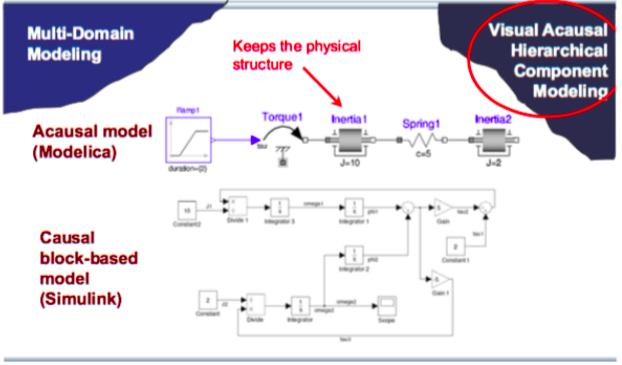
\includegraphics[width=1\linewidth]{om1}
\caption{Comparison of graphical environment of Openmodelica and Simulink \cite{PeterFrit}}
\label{fig:OM1}
\end{figure}

Being an object oriented language openmodelica also supports inheritance through which a child class can inherit the properties of a parent class. Now the child class can implement the same behavior of the parent class.

\subsection{Graphical Modelling}
Openmodelica permit users to attach their own graphics to the models. This helps in better visualization of the system. Unlike other simulation software, which exhibits just on signal flow model modelica exhibits a physical model which is easy to understand and visualize. Due to the acausal feature the user just have to connect the different models involved in the flowsheet without worrying about the signal flow. Figure \ref{fig:OM1} show a comparative system of openmodelica versus simulink.
Openmodelica offers an integrated modelling and simulation environment where one can first model the unit and then connect them with each other graphically. This relieves the user of writing the connecting equations and codes. Openmodelica has a special feature for establishing inter model connection, named connectors. Connector is a special type of class through which users can define what are the incoming or outgoing variables from a model.

Following are two types of variables that can be defined in a connector.
\begin{itemize}
\item {\textbf{Flow variables}}
Flow variables are those variables comes in or goes out of a model example the current flowing through a resister. In openmodelica flow variables follow the Kirchhoff's current law, which means the total amount of any quantity coming into any node is equal to the amount of quantity going out of that node.
\item{\textbf{Potential variables}}
Potential variables are variables that replicates the voltage in an electrical circuit. In openmodelica, potential variables follow Kirchhoff's voltage law, which states that the directed sum of the variables around any closed loop should be zero.
\end{itemize}

Openmodelica offers an excellent graphical facility which is drag and drop composition. Using this one can easily drag and drop models to the simulation environment and connect them through a mouse cursor. Figure \ref{Dist} depicts this feature of open modelica.

\begin{figure}
\centering
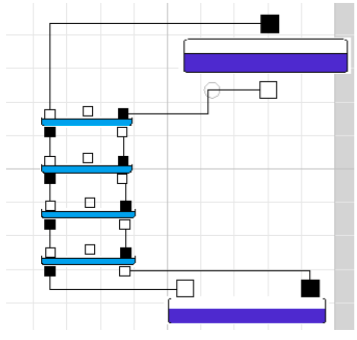
\includegraphics[width = 0.6\linewidth]{Dist}
\caption{A distillation tower model as a connection of tray model in openmodelica}
\label{Dist}
\end{figure}

\section{Drawbacks}
\begin{itemize}
\item {As modelica is a generic modelling and simulation environment it has no built in chemical engineering unit operations.}
\item{Openmodelica does have a thermodynamic engine. Therefore thermodynamic calculations cannot be performed.}
\item{As every unit operation has to be coded user has to provide the solver with good initial guess values otherwise the model may not converge.}
\end{itemize}

\chapter{Importing the Thermodynamic engine of DWSIM in Openmodelica.}

\section{Motivation}
\begin{itemize}
\item{\textbf{Design and Optimization}} \\
As shown in chapter three DWSIM is not efficient in handling design and optimization problems because it is based on sequential modular approach but has a strong thermodynamic engine. As described earlier DWSIM also has a standalone thermodynamic library (DTL) which can be used externally. On the other hand openmodelica is apt in handling equations but lacks thermodynamics. Therefore, if somehow the thermodynamics of DWSIM is imported to openmodelica, both these problems can be solved.

\item{\textbf{Dynamic Simulation}} \\
As stated in chapter three DWSIM cannot simulate dynamic systems. On the other hand openmodelica can do this very efficiently due to its strong built in integration solvers. Again if DTL is clubbed with openmodelica, simulation of dynamic chemical processes can easily be carried out.

\end{itemize}
The above two benefits shows that it may be a fruitful exercise to integrate the DTL with openmodelica. As a result one may obtain a complete process simulator which is capable of solving all type of problems that is simulation, design, optimization with steady state or dynamic behavior.

\section{Python-C API approach to Integrate Openmodelica with DTL} \cite{api}
DTL consists of a file with an extension .dll (dynamic link library) which is written in VB.NET (windows environment). This file is COM (component object model) enabled, which means that any programming language which supports COM can import this library and access the built in thermodynamic subroutines. Openmodelica is written in C (Linux environment) and the only language whose routines can be called from openmodelica is C. As both these programs are developed in so different environment it becomes hard to integrate the two.
As openmodelica supports only C language, it would have been best to call DTL from C but unfortunately due to the difference in their environment both were not compatible. Therefore, there was a need to bring in some glue language which can establish this integration from DTL to C. For this purpose python was chosen as it is an excellent glue language.

The package \textbf{win32com} in python can be used to establish connection with COM enabled objects. Therefore, using win32com we can call the DTL library and hence all the thermodynamic routines available in it.

Python-C API is one of the approach through which this integration of openmodelica and DTL is carried out successfully. Figure \ref{PyC1} describes the flow of the approach. Following points describes the structure and flow of this approach \ref{appenA}.

\begin{figure}
\centering
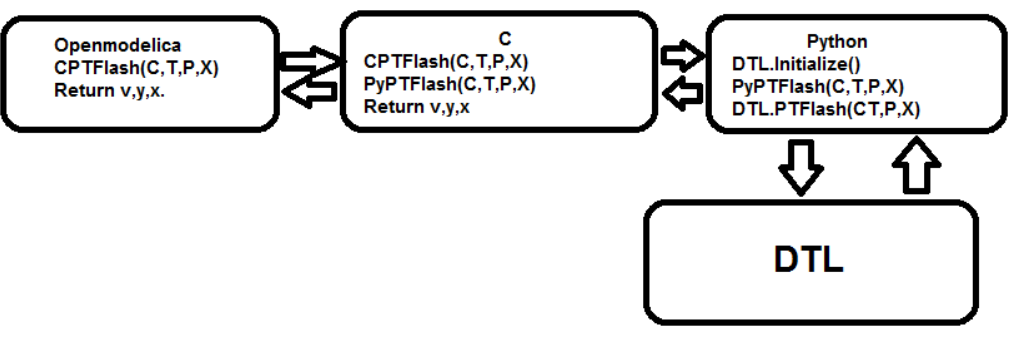
\includegraphics[width=1\linewidth]{PytC1}
\caption{Structure of Python-C API approach}
\label{fig:PyC1}
\end{figure}
\begin{itemize}
\item{First the DTL routines were imported to python. A package in python named win32com.client was used to do that. This package allows python to call routines from a dll file which is registered in the windows registry. Once the dll file is dispatched through win32com.client, python has access to all the COM enabled functions of the dll.}
\item{Once DTL is imported to python now python functions were written to send input parameters to DTL routines and calculate the required thermodynamic properties. These python functions now behaves similarly as DTL routines. The codes for python functions are shown in appendix A.}
\item{These python functions are now called by C through python-C API. In computer programming, an API (Application programming interface) is a set of routines, protocols, and tools for building software applications. An API expresses a software component in terms of its operations, inputs, outputs, and underlying types. This API is responsible for converting C variables to python and vice versa. The codes for C functions are shown in Appendix A}
\item{Finally as openmodelica is compatible with C, the inputs are then sent to C functions through openmodelica external C functions, which in turn calls the python functions, which in turn calls DTL routines. The codes for external function in openmodelica are shown in Appendix A.}
\end{itemize}
\section{Client-Server (sockets) approach to integrate OpenModelica with DTL} \cite{socket}
Client-Server or socket approach is another approach through which the integration is successful. Figure \ref{PyC2} describes the data flow of the approach. Following points describes the structure and flow of this approach \ref{appenB}.

\begin{figure}
\centering
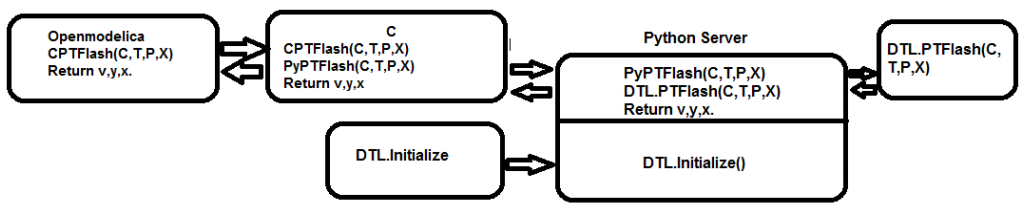
\includegraphics[width=1\linewidth]{PytC2}
\caption{Structure of Python-C socket approach}
\label{fig:PyC2}
\end{figure}

\begin{itemize}
\item{In this approach also, firstly the the DTL routines are called in python with the help of win32com.client package.}
\item{Similar to python-C approach, functions are written in python which calls DTL to calculate various physical properties.}
\item{Now a python server which consists of all the above functions is created which waits for a C clients to establish connection, receive inputs from it and send the calculated values back to the client. The codes for python server in shown in Appendix B}
\item{Clients are coded in C which establishes connections with the python servers and send and receive data from it. The codes for C client is shown in Appendix B}
\item{Once the connection is established the python server receives the data from C client, contacts DTL, calculate the required property as asked by the C client and sends it back to the client.}
\item{Finally the these C clients are called by openmodelica external C functions giving the required inputs to the client which in turn contacts the python servers for the calculation. The C client receives the calculated values from python servers and transfers it to openmodelica.}
\end{itemize}

\section{Implementation of the two approaches}
Table \ref{Prop} lists the thermodynamic functions and their that can be used in openmodelica to receive values from DTL. These functions can be used directly in any simulation. 

When, using the socket approach the python server should be up and running during the execution of the simulation. 

These thermodynamic functions can be used along with the mass and energy balance written in openmodelica to solve the unit operation modules. 

\begin{table}
\label{Prop}
\caption{Thermodynamic routines and the procedures to call them}
\centering
\begin{tabular}{|c|c|c|} \hline
Thermodynamic Prop & Thermodynamic Funct & Arguments \\ \hline
Vapur Pressure & VapPres & Comp,T \\
Enthalpy & Ent & Comp., T,P \\
Liquid Density & LiqDen & Comp,T \\
Vapour Density & VapDen & Comp,T \\
Pres. Temp. Flash & PTFlash & Comp,Z,T,P,Model \\
Pres. Volume. Flash & PVFlash & Comp,Z,V,P,Model \\
Pres. Enth. Flash & PHFlash & Comp,Z,H,P,Model \\
Liquid Viscosity & LiqVis & Comp,T \\
Vapour Viscosity & VapVis & Comp,T \\
Surface tension & SurfTen & Comp,T \\ \hline
\end{tabular}
\end{table}

\section{Comparison of the Two Approaches}
The following two models were simulated in openmodelica with different integration approaches to import DTL.

\begin{itemize}
\item{\textbf{Steady State Flash Separator}} \\
An equimolar mixture of Benzene and Toluene was flashed in a flash separator. The thermodynamic package used was Raoult's law. All the pure component and mixture properties were imported from DTL. To test the capability of the integration methods the composition of the resulting vapor stream was specified, and the temperature at which this composition is attained was left unknown. It was observed that the \textbf{Python-C API} approach took thirty seconds to solve the system, whereas the \textbf{Client-Server} method took less than one second to simulate.
\item{\textbf{Dynamic Flash}} \\
A dynamic flash was simulated with the feed as equimolar mixture of benzene and toluene. The thermodynamic package used was again Raoult's Law. It was assumed that the output liquid stream was at the same composition and temperature, as the holdup inside the flash separator. Heat supplied to flash separator was kept constant. The set of equations involved were mass balance, energy balance and equilibrium equations. The mass and energy balance were differential equations. It was observed that the Python-C API approach took \textbf{thirty minutes} to solve, whereas the Client-Server approach takes \textbf{four minute} to solve the system.
\end{itemize}

The above two examples clearly states that Client-Server approach is much faster than Python-C API approach. This is because of two reasons.

\begin{itemize}
\item {Before you call any routine of DTL one has to call another DTL routine named Initialize. This routine loads all the compounds and their properties from the database, which consumes lot of time. In Python- C API approach this initialize routine was called every time a call was made from openmodelica to C and from C to modelica. When a model is simulated in openmodelica using DTL through Python-C API approach, on each iteration such a call was made and every time the Initialize routine was called. This repeated loading of the database through initialize make the process very slow. Whereas in Client-Server approach, before the server is ready to accept connections from client the initialize routine is already called. Therefore the initialize routine was only called once and not on every single iteration.}
\item{Whenever API is used in any program it makes it slow as there are lots of conversion involved like data type conversions etc. As python-C API approach is based on API it is slow.}
\end{itemize}

\chapter{Development of a built in Thermodynamic engine in Openmodelica.}

\section{Motivation}

The following three reasons justifies the requirement of a built in thermodynamic engine in openmodelica.

\begin{itemize}

\item The two approaches as described in the previous chapter imports DWSIM's thermodynamic engine in openmodelica. This means that the thermodynamic engine is sitting outside openmodelica and has to be called each and every time a thermodynamic property is to be calculated. This process is too time consuming, thus making it impossible to solve complex models involving rigorous thermodynamics calculations. 

\item As DWSIM's thermodynamic is external to openmodelica, it appears to be a black box to openmodelica, where inputs are send and calculated values are obtained which are solved by DWSIM's solver. Openmodelica is unable to access the thermodynamic equations and therefore it is totally unaware of the nature of these equations. On the other hand if these equations are available in openmodelica itself, they can be solved simultaneously with mass and energy balance thereby solving all the equations simultaneously using openmodelica's own solver. This seems to be lot faster as openmodelica now knows the nature of these equations and they are solved internally by openmodelica itself.

\item Another key point to be considered is as described in chapter four, openmodelica has a rich set of nonlinear and ODE solvers which are written in C. This makes the solving process too fast. Whereas DWSIM solvers are written in C\# which is slower than C in terms of computation time required. Consequently, the calculation of thermodynamic properties , which are highly nonlinear equations, is much faster in openmodelica than DWSIM. 

\item The problem with DTL approach is that as DTL is a dll file it is supported only in windows. Infact the concept of COM is only supported by windows. Therefore, this approach dosen't work in other operation systems like linux and mac. Whereas, the build in thermodynamics is a part of openmodelica itself and openmodelica is compatible with every operating system. Therefore the built in thermodynamic should be multi platform.

\end{itemize}

\section{Development of the three components of a thermodynamic engine}
\subsection{Development of Compound Database}
\begin{itemize}
\item {\textbf{The Chemsep Database}} \\
Chemsep is an open source database, written in \textbf{xml} format, of over six hundred compounds with a comprehensive set of thermodynamic properties of each compound. It also has an extensive database of binary interaction parameters for thermodynamic packages like NRTL, Peng Robinson, UNIQUAC, SRK etc. Most of the thermodynamic properties are calculated by using empirical equations which are functions of temperature or pressure. Chemsep database includes the constants which are used in these equations. Therefore, chemsep database is a comprehensive database that can be used to built a powerful and robust thermodynamic engine.

\item{\textbf{Porting Chemsep database into Openmodelica}} \\
As described in the previous section chemsep database is written in xml format. This xml data has to be re written in such a form which can be understood by openmodelica. Therefore, each compound (including all its thermodynamic properties) is replicated as a single class in openmodelica as shown in figure \ref{fig:BT1}. The properties are given abbreviations ( as shown in table \ref{tab:indprop}) so that they can be called conveniently. The conversion from xml to openmodelica classes is carried out by developing a python script (see Appendix \ref{appenC} ) which automates this process, thus making it fast and robust. 

Now, one can extract any independent property of a compound by the \textbf{.} operator followed by the property relevant abbreviation. For example the critical temperature (Tc) of methane can be accessed by \textbf{Methane.Tc}. Similarly, all the properties of any compound can be accessed in the same way as shown in table \ref{tab:indprop}. \\
\end{itemize}

\begin{figure}
\centering
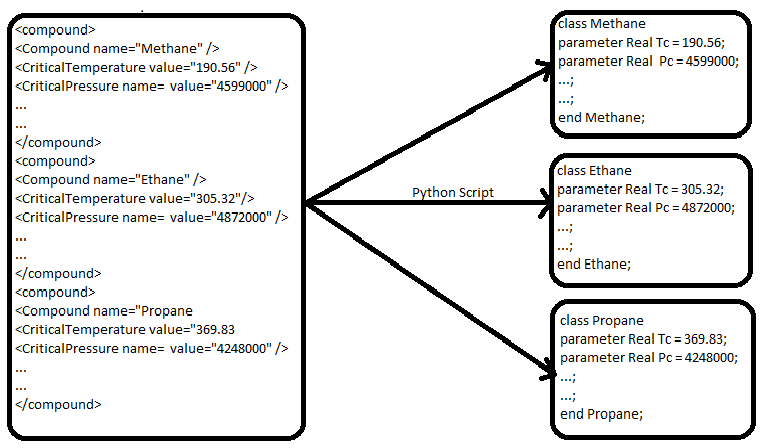
\includegraphics[width=0.8\linewidth]{BT1}
\caption{Porting chemsep database in Openmodelica}
\label{fig:BT1}
\end{figure}


\begin{table}
\centering
\caption {Independent thermodynamic properties and openmodelica routines to call them.}
\label{tab:indprop}
\vspace{1ex}
\begin{tabular}{l|l} \hline
Thermodynamic Property & Calling procedure \\ \hline
Critical Temperature & Compound.Tc \\
Critical Pressure & Compound.Pc \\
Critical Volume & Compound.Vc \\
Boiling point & Compound.Tb \\
Melting poind & Compound.Tm \\
Molecular weight & Compound.MW \\
Accentric Factor & Compound.AF \\
Triple Point & Compound.TT \\
Solubility parameter & Compound.SP \\ 
Dipole moment & Compound.DP \\ 
Heat of formation & Compound.HOF \\ 
Absolute enthalpy & Compound.ABSENT \\ \hline
\end{tabular}
\end{table}

\subsection{Development of Thermodynamic Functions}

As discussed earlier most of the thermodynamic properties of pure compounds which depends on temperature or pressure are in the form of equations which includes constants and an independent variable (temperature and pressure). These properties are written in the form of functions in openmodelica. The arguments to these functions are the independent variable (temperature, pressure, composition) and the coefficients of the respective compound whose properties have to be calculated. The coefficients can be accessed by instantiating the base compound class. The functions then returns the calculated property. For example the vapor pressure of methane at 300 K can be calculated by first instantiating the base methane class and then calling \textbf{Pvap(water.VP, 373)}. Where Pvap is a generic function to calculate the vapor pressure of any compound at any given temperature. The whole process is shown in figure \ref{fig:BT2}. Similarly, all other thermodynamic properties can be calculated using their respective functions as shown in table \ref{tab:depprop}.

\begin{figure}
\centering
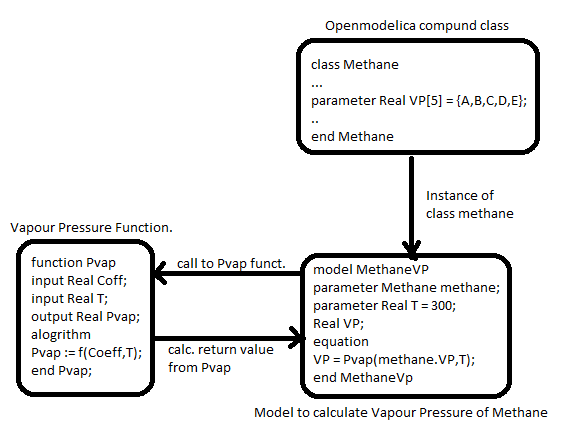
\includegraphics[width=0.8\linewidth]{BT2}
\caption{Using built in thermodynamic functions (Pvap)}
\label{fig:BT2}
\end{figure}

\begin{table}
\centering
\caption {Dependent thermodynamic properties and openmodelica functions to call them.}
\label{tab:depprop}
\vspace{1ex}
\begin{tabular}{l|l} \hline
Thermodynamic Property & Calling procedure \\ \hline
Liquid density & LiqDen(Compound name,temperature) \\
Vapor pressure & VP(Compound name,temperature) \\
Heat of Vaporization & HOV(Compound name,temperature) \\
Liquid heat capacity & LiqCp(Compound name,temperature) \\
Liquid viscosity & LiqVis(Compound name,temperature) \\
Vapor viscosity & VapVis(Compound name,temperature) \\
Liquid thermal conductivity & LiqK(Compound name,temperature) \\
Vapor thermal conductivity & VapK(Compound name,temperature) \\ \hline
\end{tabular}
\end{table}

\subsection{Development of Phase Equilibria models}
In a mixture which finds itself in a vapor-liquid equilibria state (VLE), the component fugacities are the same in all phases, that is :
\begin{align*}
f_i^L = f_i^V 
\end{align*}
The fugacity of a component in a mixture depends on temperature, pressure and composition. in order to relate fiV with temperature, pressure and molar fraction, we define the fugacity coefficient,
\begin{align*}
\Phi_i = \frac{f_i^V}{y_iP^*}
\end{align*}
which can be calculated from PVT data, commonly obtained from an equation of state. For a mixture of ideal gases, $\Phi_i$ = 1.
The fugacity of the i component in the liquid phase is related to the composition of that phase by the activity coefficient $\gamma_i$, which by itself is related to $x_i$ and standard-state fugacity $f_i^0$ by
\begin{align*}
\gamma_i = \frac{f_i^L}{x_if_i^0}
\end{align*}
The standard state fugacity $f_i^0$ is the fugacity of the i-th component in the system temperature, i.e. mixture, and in an arbitrary pressure and composition. Here, the standard-state fugacity of each component is considered to be equal to pure liquid i at the system temperature and pressure. An Equation of State is used to calculate equilibria, fugacity of the i-th component in the liquid phase is calculated by
\begin{align*}
\gamma_i = \frac{f_i^L}{x_iP^*}
\end{align*}
with the fugacity coefficient $\Phi_i$ calculated by the EOS, just like it is for the same component in the vapor phase.
The following EOS models are developed in openmodelica \cite{DWSIM}.

The binary interaction parameters for each of the EOS and acitivity coefficient models have been extracted from chemsep database where they are saved in a .dat file. The following procedure is used to port all the binary interaction parameters to openmodelica. 

\begin{itemize}
\item First, the dat file is converted to a csv file as python is very much comfortable with csv format. To accomplish this sublime editor is used which makes this task simple enough.
\item This csv is then converted to an openmodelica function by a python script (Appendix C) which converts the compound and the binary interaction parameters as an array.
\end{itemize}

\begin{figure}
\centering
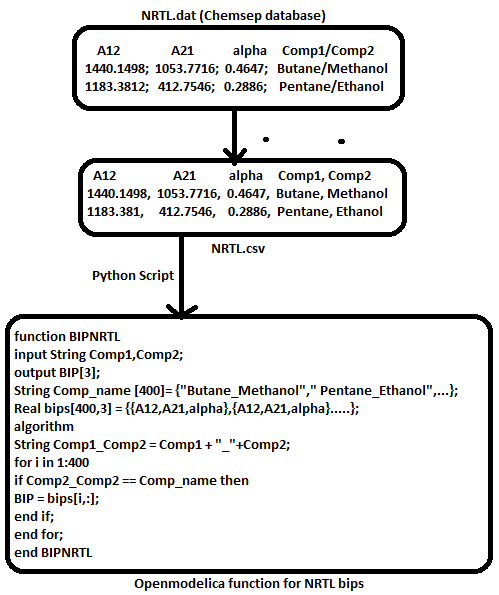
\includegraphics[width=0.8\linewidth]{BT3}
\caption{Porting Chemsep's binary interaction parameters in openmodelica}
\label{fig:BT3}
\end{figure}

Figure \ref{fig:BT3} demonstrate the above process for NRTL activity coefficient model.

\begin{itemize}
\item{\textbf{Peng Robinson}} \\
The following equations represent the Peng Robinson model \cite{PR}.
\begin{gather*}
a(T) = [1+(0.37464 + 1.54226\omega - 0.2699\omega^2)(1-T{_r}^{(1/2)})] ^20.45724(R^2T_c^2)/P_c \\
b = 0.07780(RT_c)/P_c
\end{gather*}
where \\
$\omega$  acentric factor (obtained by Compound.W) \\
$T_c$ critical temperature \\
$P_c$ critical pressure \\
$T_r$ reduced temperature, T/$T_c$ \\
\begin{gather*}
a_m = \sum_i\sum_jx_ix_j\sqrt{a_ia_j}(1-k_{ij}) \\
b_m = \sum_ix_ib_i
\end{gather*}
where \\
$x_{i,j}$ molar fraction of the i or j component in the phase (liquid or vapor) \\
$a_{i,j}$ i or j component a constant \\
$b_{i,j}$ i or j component b constant \\
$k_{i,j}$ binary interaction parameter which characterizes the i-j pair \\

The fugacity coefficient obtained with the Peng-Robinson EOS \cite{DWSIM} is given by
\begin{gather*}
ln\frac{f_i}{x_iP} = \frac{b_i}{b_m}(Z-1) - ln(Z-B) - \frac{A}{2\sqrt{2}B}(\frac{\sum_kx_ka_{ki}}{a_m} - \frac{b_i}{b_m})ln(\frac{Z+2.414B}{Z-0.414B})
\end{gather*}

where Z is the phase compressibility factor and can be obtained from 
\begin{gather*}
Z^3 - (1-B)Z^2 + (A-3B^2-2B)Z - (AB-B^2-2B) = 0 \\
A = \frac{a_mP}{R^2T^2} \\
B = \frac{b_mP}{RT} \\
\end{gather*}

\item {\textbf{Soave-Redlich-Kwong Equation of State}} \\
The Soave-Redlich-Kwong Equation \cite{SRK} is also a cubic equation of state in volume. \\
The a and b parameters are given by
\begin{gather*}
a(T) = [1 + (0.48 + 1.574\omega - 0.176\omega^2)(1-T_r^{(1/2)})]^{2}0.42747(R^2T^2)/P_c \\
b = 0.08664(RT_c)/P_c \\
\end{gather*}
The fugacity is calculated by
\begin{gather*}
ln\frac{f_i}{x_iP} = \frac{b_i}{b_m}(Z-1) - ln(Z-B) - \frac{A}{B}(\frac{\sum_kx_ka_{ki}}{a_m} - \frac{b_i}{b_m})ln(\frac{Z+B}{Z})
\end{gather*}
The phase compressibility factor Z is obtained from 
\begin{gather*}
Z^3 - Z^2 + (A - B - B^2)Z - AB = 0 \\
A = \frac{a_mP}{R^2T^2} \\
B = \frac{b_mP}{RT} \\
\end{gather*}

\item{\textbf{NRTL}}\\
Renon and Prausnitz \cite{NRTL} developed the NRTL equation (Non-Random, Two-Liquid) based on the concept of local composition but, unlike Wilsonâ  model, the NRTL model is applicable to systems of partial miscibility. The model equations are:
\begin{gather*}
ln\gamma_i = \frac{\sum_{j=1}^{n}\tau_{ji}x_jG_{ji}}{\sum_{k=1}^{n}x_kG_{ki}} + \sum_{j=1}^{n}\frac{x_jG_{ij}}{\sum_{k=1}^{n}x_kG{kj}}(\tau_{ij} - \frac{\sum_{m=1}^{n}\tau{mj}x_mG_{mj}}{\sum_{k=1}^{n}x_kG_{kj}}) \\
G_{ij} = exp(-\tau_{ij}\alpha_{ij}) \\
\tau_{ij} = \frac{\alpha_{ij}}{RT} \\
\end{gather*}
$\gamma_i$ Activity coefficient of component i \\
$x_i$ Molar fraction of component i \\
$\alpha_{ij}$ Interaction parameter between i-j ($a_{ij} = a{ji}$) (calculate/mol) \\
T Temperature (K) \\
$\alpha_{ij}$ non-randomness parameter for the i-j pair ($a_{ij} = a{ji}$)

\end{itemize}

\chapter{Implementation of the built in thermodynamics in Openmodelica}
The following example demonstrates the implementation of the built in thermodynamics in openmodelica.

\section{Steady state flash of ethanol-water system}
\subsection{The Model}
An equimolar feed containing ethanol and water is to be flashed at 1 atm and 355 K. The resulting vapour and liquid compositions are to be calculated. Following are the modelling equations for the same. 


\begin{gather*}
\intertext{Mass balance}
z_iF = x_iL + y_iV 
\intertext{for i = 1,2}
\intertext{Where}
\intertext{F,L,V  feed,liquid,vapour flowrate resp. (100kmol/hr)}
\intertext{$z_i,x_i,y_i$ feed,liquid,vapour compositions resp.}
\end{gather*}

Equilibrium equations
\begin{gather*}
y_i = K_ix_i \\
\intertext{for i = 1,2} \\
\end{gather*}
Where \\
$K_i$ is the equilibrium constant obtained from UNIQUAC model. \\
Summation Equation \\
\begin{gather*}
\sum_{i=1}^2y_i = 1
\end{gather*}   

UNIQUAC activity coefficient model is used as the phase equilibria model. 
 
\subsection{Openmodelica code and its explanation}

\begin{figure}
\centering
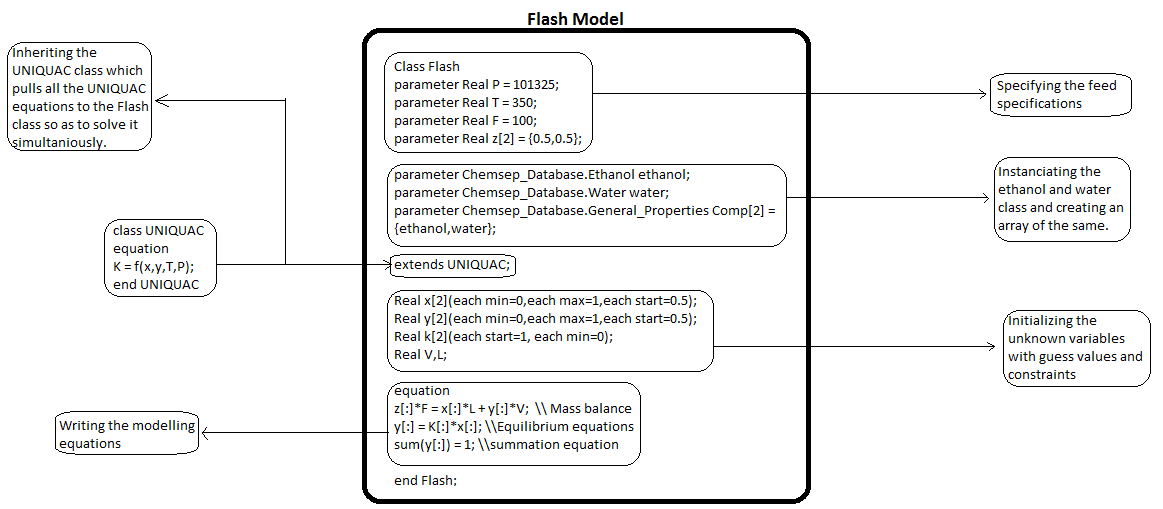
\includegraphics[width=1.2\linewidth]{omcode}
\caption{Openmodelica code for ethanol-water flash.}
\label{omcode}
\end{figure}

Figure \ref{omcode} describes the code used to simulate the flash. The first four lines specifies variables which carries the feed specifications (temperature, pressure, composition, flowarate). The next set of lines instanciate the compound class ethanol and water and creates an array of the same. The next line \textbf{extends UNIQUAC} is used to inherit the already developed UNIQUAC class (which has all the equations for UNIQUAC model). By inheriting a class all the equations and variables of the inherited class are actually dragged and added to the class which inherits it. Therefore, all the UNIQUAC equations are added to the equation section of the Flash class. The next set of variables initializes and defines the unknown variables that needs to be calculated. Finally, the equation section has all the modelling equations required for the simulation of the flash. 

\subsection{How openmodelica handles and solves the model equations}
As described in chapter 5, openmodelica follows an equation oriented approach where all the equations are solved simultaneously. Referring to the above example openmodelica collects all the model equations along with the thermodynamic equations (UNIQUAC equations in this case) and then solves them simultaneously. The fact that thermodynamic equations are solved simultaneously along with the modelling equations can be shown by executing the transformational debugger which shows all the equations that are to be solved simultaneously. Figure \ref{TD} shows the snapshot of the transformational debugger for the above flash example. It can be seen that the all the equations irrespective of their type (thermodynamic or mass balance) are solved simultaneously.

By default openmodelica uses \textbf{Dassl} to solve differential algebric equations and a hybrid solver for solving algebraic equations. However, we can choose a different solver from the list of solvers. This is achieved by going in the simulation setup window, where one can specify all the details regarding the simulation for example the time period, the number of intervals for simulation etc. The output of openmodelica's successful simulation is a mat or a csv file.

\begin{figure}
\centering
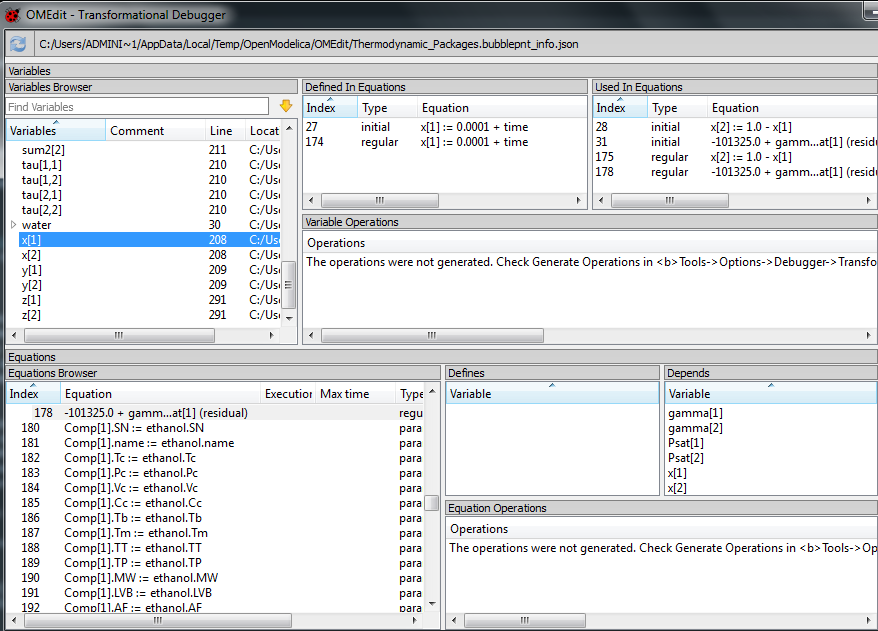
\includegraphics[width=0.9\linewidth]{TD}
\caption{Snapshot of transformational debugger in openmodelica.}
\label{TD}
\end{figure}

\chapter{Solved examples in Openmodelica using the built in thermodynamics}

\section{Generating VLE curve (Txy) for ethanol water system using the UNIQUAC model.}

\begin{itemize}
\item {\textbf{Bubble point}} \\
Modified Roult's law (equations \ref{eqn:RL2}) is the governing equation to generate the bubble point curve.

\begin{align}
y_1.P = \gamma_1.x_1.Pvap_1 \label{eqn:RL1}\\
y_2.P = \gamma_2.x_2.Pvap_2 \label{eqn:RL2} 
\intertext{where $\gamma_1$ and $\gamma_2$ are activity coefficients. $y_1$, $y_2$ are vapor phase compositions. $x_1$, $x_2$ are liquid phase compositions and $Pvap_1$, $Pvap_2$ are corresponding vapor pressures.
Adding the above two equations and putting $y_1$ + $y_2$ = 1 we get} \nonumber \\
P = \gamma_2.x_2.Pvap_2 + \gamma_1.x_1.Pvap_1 \label{eqn:RL3}
\intertext{Here $\gamma_1$ and $\gamma_2$ are complex nonlinear functions of temperature and liquid compositions and $Pvap_1$ and $Pvap_2$ are functions of temperature} \nonumber
\end{align} 

The pressure is kept constant at 1 atm. The value of $x_1$ (mole fraction of ethanol) is varied from 0 to 1 with an interval of 0.1 and for each value of $x_1$ the corresponding value of temperature is calculated by equation \ref{eqn:RL3}. Figure \ref{fig:BP} shows the resulting tx curve as calculated by the developed built in thermodynamics in openmodelica.

\begin{figure}[t]
\centering
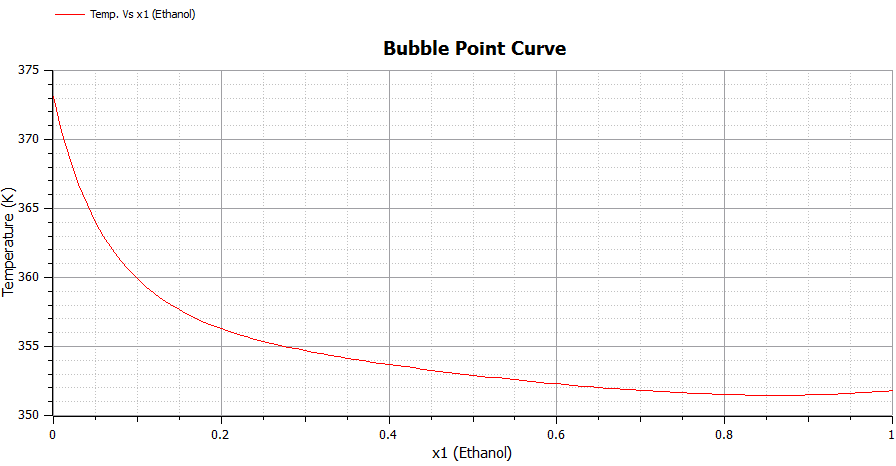
\includegraphics[width=0.8\linewidth]{BP}
\caption{Bubble point (Tx) curve for ethanol water system generated in openmodelica.}
\label{fig:BP}
\end{figure}

\item {\textbf{Due point}} \\
Modified Roult's law (equations \ref{eqn:RL2}) is the governing equation to generate the dew point curve.

\begin{align}
\intertext{Manipulating the equations \ref{eqn:RL1} and \ref{eqn:RL2} and putting $x_1$ + $x_2$ = 1 we get} \nonumber \\
\frac{y_1}{\gamma_1.Pvap_1} + \frac{y_2}{\gamma_2.Pvap_2}  = 1 \label{eqn:RL4}
\end{align} 

The pressure is kept constant at 1 atm. The value of $y_1$ (mole fraction of ethanol) is varied from 0 to 1 with an interval of 0.1 and for each value of $y_1$ the corresponding value of temperature if calculated by equation \ref{eqn:RL4}. Figure \ref{fig:DP} shows the resulting ty curve as calculated by the developed built in thermodynamics in openmodelica.

\begin{figure}[t]
\centering
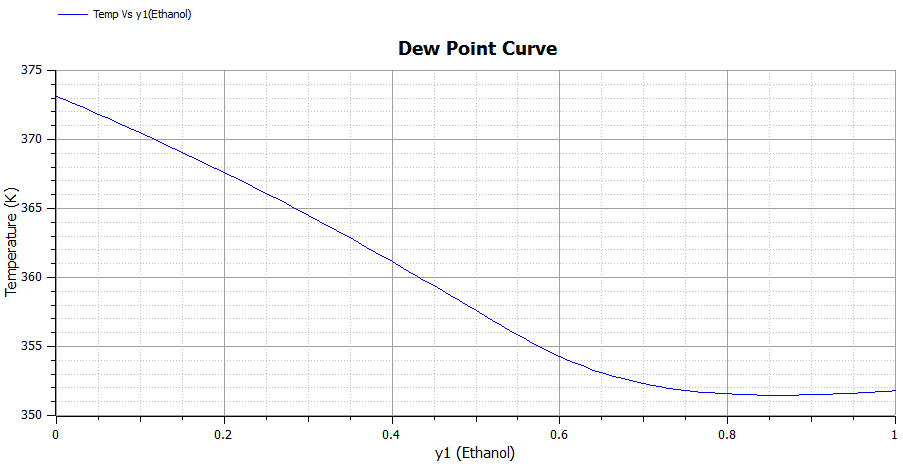
\includegraphics[width=0.8\linewidth]{DP}
\caption{Dew point (Ty) curve for ethanol water system generated in openmodelica.}
\label{fig:DP}
\end{figure}

\item Combining the bubble point and the dew point curves as generated above gives the Txy curve for the system as shown in Figure \ref{fig:VLE}
\begin{figure}
\centering
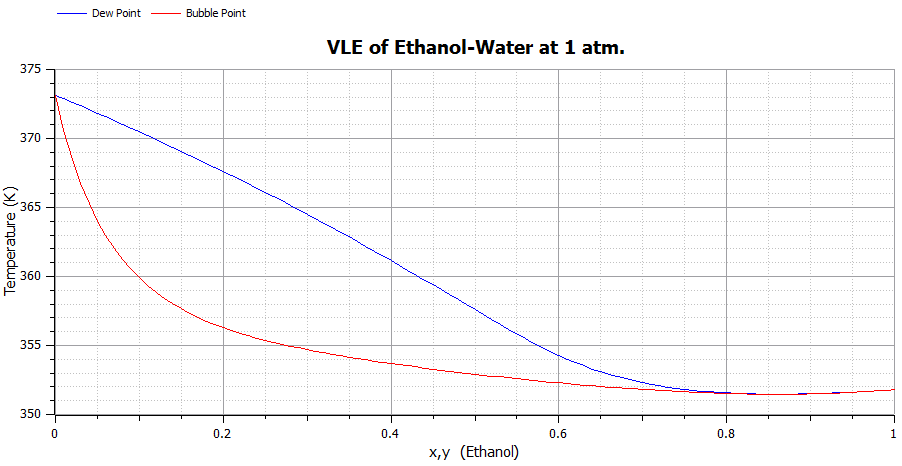
\includegraphics[width=0.8\linewidth]{VLE}
\caption{Txy curve for ethanol water system generated in openmodelica}
\label{fig:VLE}
\end{figure}

This figure is verified by reproducing the same problem in Aspen plus. Figure \ref{aspen} depicts the Txy curve for ethanol water system generated in Aspen plus. It clearly shows that the plot generated in openmodelica completely replicates the one generated in Aspen plus. 

Reliable azeotropic data source by American Chemical Society \cite{Az} says that for ethanol-water system, at 1 atm, the azeotropic composition and temperatures are 0.96 mole fraction ethanol and 351.4 K. These values are also in agreement with the openmodelica results.

\begin{figure}
\centering
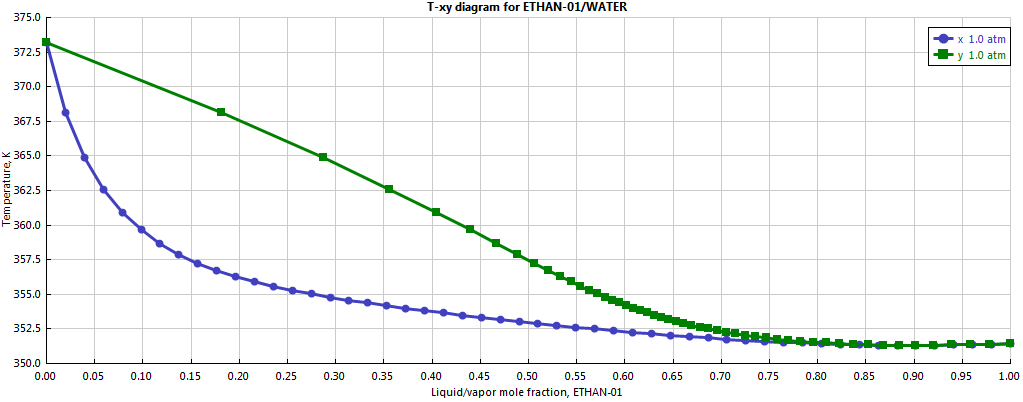
\includegraphics[width=0.9\linewidth]{aspen}
\caption{Txy curve for ethanol-water system (UNIQUAC) generated in Aspen Plus}
\label{aspen}
\end{figure}

The same simulation when carried out with the imported DWSIM's thermodynamic engine in openmodelica resulted in an execution time of about 20 minutes whereas for the built in thermodynamic engine the execution time was fraction of a second.  

\end{itemize}
\section{Steady State Flash}
\subsection{The Model}
In this model a steady state flash is simulated in openmodelica using the developed thermodynamics. The components involved are methanol, ethanol and water. The thermodynamic package used is NRTL. To check the design efficiency of the developed thermodynamic engine in openmodelica , the output composition of the vapor product is specified, while the temperature at which this desired composition of vapor is attained needs to be calculated. Therefore, it is a design problem. To carry out this simulation in DWSIM, we have to use an adjust operation which uses a trial and error method and is time consuming.

\subsection{Problem Statement}
The flowrate and the composition of the feed is specified. Pressure is kept constant at 1 atm. The problem is divided into three parts with each having different desired vapor compositions. The temperature and all the unknowns compositions and flow rates need to be calculated. The schematic of the problem statement is shown in figure \ref{Flash}.

\begin{figure}
\centering
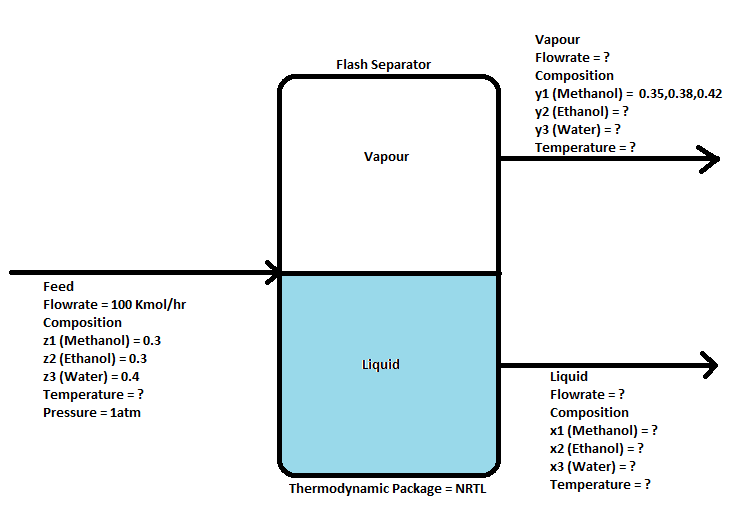
\includegraphics[width=0.8\linewidth]{Flash}
\caption{Model with problem statement for steady state flash of Methanol-ethanol-water.}
\label{Flash}
\end{figure}


\subsection{Simulation Details and Equations}
The input stream enters at 1 atm and the temperature is to be determined according to the desired vapor composition. The simulation was run for three different vapor compositions. The minimum and maximum temperatures were taken to be boiling points of pure benzene and toluene and the initial guess for temperature is taken to be average of the two boiling points. The following equations describe the model.

\begin{gather*}
\intertext{Material Balances} \\
F=V+L \\
x_{i,F}F = y_iV + x_iL \\
\intertext{For i = 1,2,3} \\
\intertext{Equilibrium relations} \\
y_i = K_ix_i \\
\intertext{For i = 1,2,3} \\
\intertext{Summation Equation} \\
\sum_{i=1}^{3}x_i = 1 \\
\intertext{Where i is the component index. y is the mole fraction in vapor phase and x in the liquid phase. 1,2,3 represents methanol, ethanol and water respectively.}
\end{gather*}

\subsection{Results}
For the three case studies the desired vapor composition is different for each case. According to the VLE behavior the case with richest vapor composition (of more volatile component) should have the lowest temperature and the case with least vapor composition (of more volatile composition) should have the highest temperature. Table \ref{Tab:Flash} show the resulting temperature and other compositions for the three different cases. The simulation time taken was almost instant, whereas if DWSIM was used it takes fifteen to twenty seconds to simulate the same.

\begin{table}
\centering
\caption{Temperature and liquid phase composition of benzene}
\vspace{1ex}
\label{Tab:Flash}
\begin{tabular}{|c|c|c|} \hline
Desired Vapor Comp. & Temperature & Liquid Comp. \\ \hline
0.6 & 369.054 & 0.378 \\
0.65 & 367.49 & 0.428 \\
0.7 & 365.842 & 0.4831 \\ \hline
\end{tabular}
\end{table}



\section{Semi-Batch Steam Distillation of a Binary Organic Mixture}
\subsection{Problem background}
This illustrative example involves semi-batch steam distil- lation of binary mixture. A schematic plot of the steam distillation apparatus is shown in Figure \ref{SD}. The organic mixture is charged into the still initially, and then steam is bubbled through continuously until the desired degree of separation has been reached. There are two different periods in the operation of the still: the heating period, until the boiling point temperature of the organic mixture is reached, and the distillation period. A brief description of the mathematical models for the two periods follows \cite{PHD}.

\begin{figure}
\centering
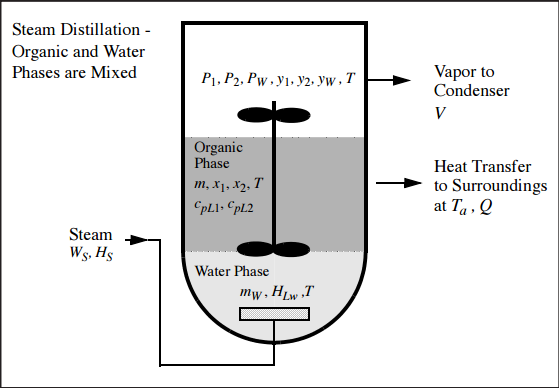
\includegraphics[width=0.8\linewidth]{SD}
\caption{Schematic of steam distillation apparatus \cite{PDH}.}
\label{SD}
\end{figure}

\textbf{Heating period} \\
A simple mass balance on the water phase yields
\begin{gather*}
\frac{dm_w}{dt} = W_s 
\end{gather*}
where $W_s$ is the steam  ow-rate in kmol/s and m is the mass SW
of water in the still in kmol. It is assumed that all the steam condenses in the distillation vessel and that the organic phase masses remain constant during the heating period.

An energy balance on the still provides the equation for the change of the temperature T in \degree C
\begin{gather*}
\frac{dT}{dt} = \frac{W_s(H_s-H_{lw}) - Q}{m_wc_{pLw}+m(x_1c_{pL1}+x_2c_{pL2})}
\end{gather*}
where $H_s$ is the enthalpy of the steam in J/kmol, HLw is the enthalpy of liquid water in J/kmol, Q is the rate of heat transfer to the surroundings in J/s, $c_{pLw}$ is the molar speci c heat of the water in J/kmol·K, m is the mass of the organic phase in the still in kmol, $x_1$ and $x_2$ are the mole fractions, and $c_{pL1}$ and $c_{pL2}$ are the molar speci c heats of organic compounds No. 1 and 2, respectively, in J/kmol·K. The heat transfer rate to the surroundings is calculated from the following equation.
\begin{gather*}
Q = UA(T - T_a)
\end{gather*}
where UA is the product of the overall heat transfer coef cient U and the contact area A with the surroundings in J/s·K, $T_a$ is the ambient temperature in K, and T is the temperature of the liquid in the still in K.

Assuming ideal liquid behavior, Raoult’s law can be used to calculate the vapor mole fraction of the components in the organic phase

\begin{gather*}
y_1 = \frac{x_1P_1}{P} \\
y_2 = \frac{x_2P_2}{P}
\end{gather*}

where P is the total pressure in Pa and $P_1$ and $P_2$ are the vapor pressures of the organic compounds in Pa. The mole fraction of the water which is immiscible in the organic phase is given by $y_W=P_W/P$. The heating period continues until the sum of vapor pressures of the organic compounds and the water is equal to the total pressure. Thus, the bubble point equation to be satis ed can be expressed as
\begin{gather*}
f(T) = 1 - (y_1+y_2+y_w) = 0
\end{gather*}

\textbf{Distillation Period} \\
During the distillation period, there is output of water vapor from the still. 
\begin{gather*}
\frac{dm_w}{dt} = W_s - Vy_w
\end{gather*}
where V is the outlet vapor  ow rate. Material balances on the two organic compounds yield two additional differential equations
\begin{gather*}
\frac{d(mx_1)}{dt} = -Vy_1 \\
\frac{d(mx_2)}{dt} = -Vy_2
\end{gather*}
The organic mass in the still at any time is given by: $m = m_x1 + m_x2$. The temperature in the still changes in a manner so that the bubble point equation is satisfied. The energy balance at a particular temperature yields the momentary vapor flow rate
\begin{gather*}
V = \frac{W_s(H_S-H{LW}) - Q}{Hv-[y_wh_{lw}+(y_1h_{L1}+y_2h_{L2})]}
\end{gather*}
where $H_V$ is the molar enthalpy of the vapor phase; $h_{Lw}, h_{L1}, and h_{L2}$ are the liquid phase molar enthalpies of water, n-octane and n-decane, respectively. Material balances on the water and organic phases in the still can provide the amount and the mole fractions of the various components in the distillate.

\subsection{Problem Statement} 
semi-batch steam distillation of an n-octane (comp. 1) and n-decane
(comp. 2) mixture. Initially M = 0.015 kmol of organics with
composition $x_1$ = 0.725 is charged into the still. The initial
temperature in the still is $T_0$ = 25 \degree C. Starting at time t = 0, steam at a temperature Tsteam = 99.2 \degree C is bubbled continuously through the organic phase at the rate of $M_S$ = 3.85e-5 kmol/s. All the steam is assumed to condense during the heating period. The ambient temperature is $T_E$ = 25 \degree C and the heat transfer coefficient between the still and the surrounding is UA = 1.05 J/s-K. The ambient pressure is P = 9.839E+04 Pa.
Assumptions: 1) Ideal behavior of all components in pure state or mixture; 2) complete immiscibility of the water and the organic phases; 3) ideal mixing in the boiler; and 4) equilibrium between the organic vapor and its liquid at all times. The standard state for enthalpy calculations pure liquids at 0 \degree C and 1 atm. can be used.

\begin{itemize}
\item Calculate and plot the still temperature (T), component mole fractions inside the still ($x_1, x_2, y_1, and y_2$), and the component mole fractions in the distillate ($x_1dist and x_2dist$) using the data and the initial values provided.
\item Determine the lowest n-octane mole fraction in the
feed that can yield a distillate concentration of $90\%$ of n-octane. Compute the percent recovery of n-octane in the distillate as function of its concentration in the feed. Vary the feed concentration in the range where the requirement for the n-octane concentration in the distillate is attainable.
\end{itemize}

\subsection{Results}
Plots \ref{SD1} and \ref{SD2} shows the results obtained by simulating the example in openmodelica by using the built in thermodynamics. \\
\begin{figure}
\centering
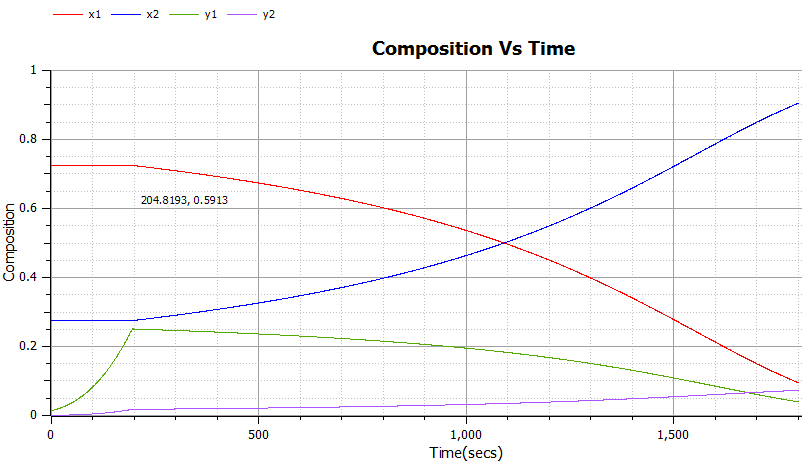
\includegraphics[width=0.8\linewidth]{SD1}
\caption{Change of organic phase composition during semi-batch steam distillation (as simulated in Openmodelica )}
\label{SD1}
\end{figure}
\begin{figure}
\centering
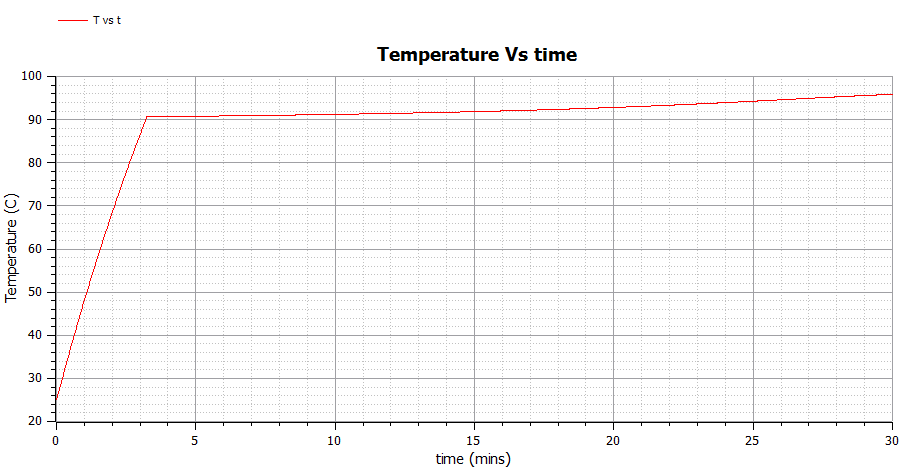
\includegraphics[width=0.8\linewidth]{SD2}
\caption{Temperature change during semi-batch steam distillation (as simulated in Openmodelica)}
\label{SD2}
\end{figure}
Plots \ref{SD3} and \ref{SD4} shows the results from the actual thesis.
\begin{figure}
\centering
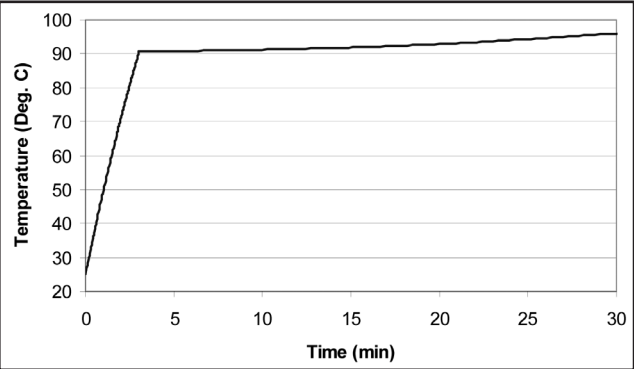
\includegraphics[width=0.7\linewidth]{SD3}
\caption{Change of organic phase composition during semi-batch steam distillation (actual thesis)}
\label{SD3}
\end{figure}
\begin{figure}
\centering
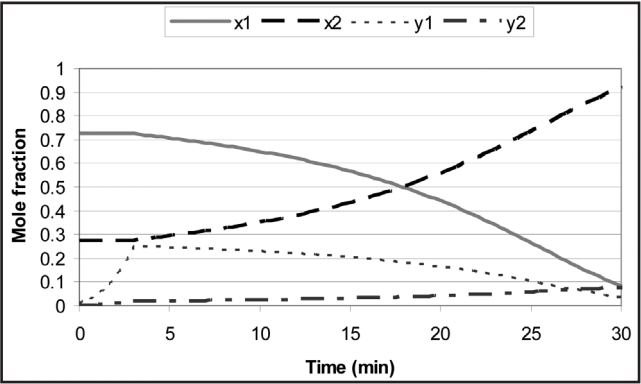
\includegraphics[width=0.7\linewidth]{SD4}
\caption{Temperature change during semi-batch steam distillation (actual these)}
\label{SD4}
\end{figure}

It can be seen that the results of openmodelica are in agreement with the original thesis. Therefore, the built in thermodynamics can be claimed to be robust and accurate.

\chapter{Future Work}
One of the next objective will be to built a library of steady state and dynamic unit operations in openmodelica. As now openmodelica has its own thermodynamic engine, a library of steady state unit operations should be modeled. Another prime objective is to build a library of dynamic unit operations in openmodelica to carry out calculations of batch processes.

After developing the unit operation library, a GUI should be developed so that an end user could conveniently use the software without getting into the complexities of the code. The GUI will be a replication of the commercial process simulators so the it might be easy for the users to adapt.

A collection of sample examples from various reliable sources should be simulated so as to verify the developed simulator, thus making it flawless. These sources might include examples from standard chemical engineering books and sample problems from commercial simulators like aspen plus.

Another objective is to identify dynamic simulation problems of interest to chemical industry and coding them in OpenModelica. An industrial campaign is planned, to visit small scale industries, who can't afford consultancy services from big consulting firms using commercial simulators, to identify their problems and provide an efficient solution as now we have an open source simulator that can handle dynamic simulations as well.

\appendix
\chapter{Codes for Python-C API Approach}
\label{appenA}
\section{The Python Code}
\begin{lstlisting}[language=Python]
def Properties(Comp,Prop,PropType,TorP):
import win32com. client
dtlc = win32com.client.Dispatch(DTL.Thermodynamics.Calculator€) dtlc . Initialize ()
if PropType==constProp€:
elif
elif
PROPVALUE = dtlc.GetCompoundConstProp(Comp,Prop) PropType==€constPDepProp€ :
TorP=float (TorP)
PROPVALUE = dtlc.GetCompoundPDepProp(Comp,Prop,TorP)
PropType==”constTDepProp” : TorP=float (TorP)
PROPVALUE = dtlc.GetCompoundTDepProp(Comp,Prop,TorP) pv = float(PROPVALUE)
return pv
def TwoPhaseProperties(PropPack,FlashAlg,P,T,Comp1,Comp2,mf1,mf2,k,l2):
import win32com. client
dtlc = win32com.client.Dispatch(”DTL.Thermodynamics.Calculator”
	dtlc . Initialize () Compounds=[”12” ,”12”]
MoleFractions=[”12” ,”12”]
pv=[[1.0 ,1.0 ,1.0 ,1.0] ,[1.0 ,1.0 ,1.0 ,1.0] ,[1.0 ,1.0 ,1.0 ,1.0]] x=[[1.0 ,1.0 ,1.0 ,1.0] ,[1.0 ,1.0 ,1.0 ,1.0] ,[1.0 ,1.0 ,1.0,1.0]] 
Compounds[0] = Comp1
Compounds [ 1 ] = Comp2
MoleFractions [0]=mf1
MoleFractions [1]=mf2
FlashAlg=float (FlashAlg)
P=float(P)
T=float(T)
l=len ( MoleFractions ) for i in range(l):
MoleFractions[ i ]= float(MoleFractions[ i ]) val=dtlc.PTFlash(PropPack, FlashAlg, P, T,Compounds, MoleFractio pv[0] = val[1]
pv[1]= val [2]
pv[2]= val [3]
for i in range(3):
for j in range(4):
x[ i ][ j]=float(pv[ i ][ j ])
return x[k][l2]
def BinaryInteractionParameters(PropPack,Comp1,Comp2,l2): import win32com. client
dtlc = win32com.client.Dispatch(€DTL.Thermodynamics.Calculator”) dtlc . Initialize ()
x=[1.0 ,1.0 ,1.0]
l2=int ( l2 )
val=dtlc . GetInteractionParameterSet (PropPack ,Comp1,Comp2)
for i in range(3):
x[i]= float(val[i])
return x[l2]
\end{lstlisting}

\section{The C Code}
\begin{lstlisting}[language=C]
#include "C:\Python27\include\Python.h"

double Property(char *Comp, char *Prop, char *PropType, double TorP)
{
	PyObject *pName, *pModule, *pDict, *pFunc, *pValue, *pTorP, *ptype, *pArgs, *pcomp, *pprop;
	double mw = 0.0;

	// Initialize the Python Interpreter
	Py_Initialize();

	// Build the name object
	pName = PyString_FromString("py_function");

	// Load the module object
	pModule = PyImport_Import(pName);

	// pDict is a borrowed reference 
	pDict = PyModule_GetDict(pModule);
	pFunc = PyDict_GetItemString(pDict, "Properties");

	// pFunc is also a borrowed reference 
	if (PyCallable_Check(pFunc))
	{
		// Prepare the argument list for the call

		pArgs = PyTuple_New(4);
		ptype = PyString_FromString(PropType);
		pcomp = PyString_FromString(Comp);
		pprop = PyString_FromString(Prop);
		pTorP = PyFloat_FromDouble(TorP);
		PyTuple_SetItem(pArgs, 0, pcomp);
		PyTuple_SetItem(pArgs, 1, pprop);
		PyTuple_SetItem(pArgs, 2, ptype);
		PyTuple_SetItem(pArgs, 3, pTorP);

		pValue = PyObject_CallObject(pFunc, pArgs);
		mw = PyFloat_AsDouble(pValue);

		if (pArgs != NULL)
		{
			Py_DECREF(pArgs);
		}

		else
		{
			pValue = PyObject_CallObject(pFunc, NULL);
		}

		if (pValue != NULL)
		{
			Py_DECREF(pValue);
		}
		else
		{
			PyErr_Print();
		}

		// some code omitted...
	}
	// Clean up
	Py_DECREF(pModule);
	Py_DECREF(pName);
	return mw;
	// Finish the Python Interpreter
	Py_Finalize();


}

double TwoPhaseProperty(char *propPack, double flashAlg, double pressure, double temp, 
char *comp1, char *comp2, double mf1, double mf2, double i, double j)
{
	PyObject *pName, *pModule, *pDict, *pFunc, *pValue, *palg, *pArgs, 
*pcomp1, *pcomp2, *pmf1, *pmf2, *ptemp, *ppres, *ppack, *pi, *pj;
	double mw = 0.0;
	// Initialize the Python Interpreter
	Py_Initialize();

	// Build the name object
	pName = PyString_FromString("py_function");

	// Load the module object
	pModule = PyImport_Import(pName);

	// pDict is a borrowed reference 

	pDict = PyModule_GetDict(pModule);
	pFunc = PyDict_GetItemString(pDict, "TwoPhaseProperties");

	// pFunc is also a borrowed reference 
	if (PyCallable_Check(pFunc))
	{
		// Prepare the argument list for the call

		pArgs = PyTuple_New(10);
		ppack = PyString_FromString(propPack);
		palg = PyFloat_FromDouble(flashAlg);
		ppres = PyFloat_FromDouble(pressure);
		ptemp = PyFloat_FromDouble(temp);
		pcomp1 = PyString_FromString(comp1);
		pcomp2 = PyString_FromString(comp2);
		pmf1 = PyFloat_FromDouble(mf1);
		pmf2 = PyFloat_FromDouble(mf2);

		pi = PyInt_FromLong(i);
		pj = PyInt_FromLong(j);

		PyTuple_SetItem(pArgs, 0, ppack);
		PyTuple_SetItem(pArgs, 1, palg);
		PyTuple_SetItem(pArgs, 2, ppres);
		PyTuple_SetItem(pArgs, 3, ptemp);
		PyTuple_SetItem(pArgs, 4, pcomp1);
		PyTuple_SetItem(pArgs, 5, pcomp2);
		PyTuple_SetItem(pArgs, 6, pmf1);
		PyTuple_SetItem(pArgs, 7, pmf2);
		PyTuple_SetItem(pArgs, 8, pi);
		PyTuple_SetItem(pArgs, 9, pj);


		pValue = PyObject_CallObject(pFunc, pArgs);
		mw = PyFloat_AsDouble(pValue);

		if (pArgs != NULL)
		{
			Py_DECREF(pArgs);
		}

		else
		{
			pValue = PyObject_CallObject(pFunc, NULL);
		}

		if (pValue != NULL)
		{

			Py_DECREF(pValue);
		}
		else
		{
			PyErr_Print();
		}

		// some code omitted...
	}
	// Clean up
	Py_DECREF(pModule);
	Py_DECREF(pName);

	return mw;
	// Finish the Python Interpreter
	Py_Finalize();

}


double binaryInteractionParameters(char *propPack, char *comp1, char *comp2, double i)
{
	PyObject *pName, *pModule, *pDict, *pFunc, *pValue, *pArgs, *pcomp1, *pcomp2, *ppack, *pi;
	double mw = 0.0;
	// Initialize the Python Interpreter
	Py_Initialize();

	// Build the name object
	pName = PyString_FromString("py_function");

	// Load the module object
	pModule = PyImport_Import(pName);

	// pDict is a borrowed reference 

	pDict = PyModule_GetDict(pModule);
	pFunc = PyDict_GetItemString(pDict, "BinaryInteractionParameters");

	// pFunc is also a borrowed reference 
	if (PyCallable_Check(pFunc))
	{
		// Prepare the argument list for the call

		pArgs = PyTuple_New(4);
		ppack = PyString_FromString(propPack);
		pcomp1 = PyString_FromString(comp1);
		pcomp2 = PyString_FromString(comp2);
		pi = PyInt_FromLong(i);

		PyTuple_SetItem(pArgs, 0, ppack);
		PyTuple_SetItem(pArgs, 1, pcomp1);
		PyTuple_SetItem(pArgs, 2, pcomp2);
		PyTuple_SetItem(pArgs, 3, pi);


		pValue = PyObject_CallObject(pFunc, pArgs);
		mw = PyFloat_AsDouble(pValue);

		if (pArgs != NULL)
		{
			Py_DECREF(pArgs);
		}

		else
		{
			pValue = PyObject_CallObject(pFunc, NULL);
		}

		if (pValue != NULL)
		{
			printf("Return of call : %d\n", PyInt_AsLong(pValue));
			Py_DECREF(pValue);
		}
		else
		{
			PyErr_Print();
		}

		// some code omitted...
	}
	// Clean up
	Py_DECREF(pModule);
	Py_DECREF(pName);

return mw;
	// Finish the Python Interpreter
	Py_Finalize();
	

}
double antoine2(char *comp, double i)
{
	PyObject *pName, *pModule, *pDict, *pFunc, *pValue, *pArgs, *pcomp, *pi;
	double mw = 0.0;
	// Initialize the Python Interpreter
	Py_Initialize();

	// Build the name object
	pName = PyString_FromString("py_function");

	// Load the module object
	pModule = PyImport_Import(pName);

	// pDict is a borrowed reference 

	pDict = PyModule_GetDict(pModule);
	pFunc = PyDict_GetItemString(pDict, "antoine");

	// pFunc is also a borrowed reference 
	if (PyCallable_Check(pFunc))
	{
		// Prepare the argument list for the call

		pArgs = PyTuple_New(2);
		pcomp = PyString_FromString(comp);
		pi = PyInt_FromLong(i);

		PyTuple_SetItem(pArgs, 0, pcomp);
		PyTuple_SetItem(pArgs, 1, pi);


		pValue = PyObject_CallObject(pFunc, pArgs);
		mw = PyFloat_AsDouble(pValue);

		if (pArgs != NULL)
		{
			Py_DECREF(pArgs);
		}

		else
		{
			pValue = PyObject_CallObject(pFunc, NULL);
		}

		if (pValue != NULL)
		{

			Py_DECREF(pValue);
		}
		else
		{
			PyErr_Print();
		}

		// some code omitted...
	}
	// Clean up
	Py_DECREF(pModule);
	Py_DECREF(pName);

	return mw;
	// Finish the Python Interpreter
	Py_Finalize();

}

double calcP(char *comp, char *property, char *propType, double T0){
	double guess[6], Tguess[6], P;
	int i;
	guess[1] = 132300;
	guess[0] = 122310;
	/*clock_t time1 =clock();
	clock_t end;
	printf("%f", time1);*/
	for (i = 0; i < 2; i++)
	{
		Tguess[i] = Property(comp, property, propType, guess[i]);
		/* end = clock();
		printf("time ra time: %f\n", ((double)(end -	time1)) / CLOCKS_PER_SEC);*/
	}

	for (i = 2; i < 6; i++){
		if (fabs(Tguess[i - 1] - 339) > 0.01){
			guess[i] = guess[i - 1] - (Tguess[i - 1] - T0) * ((guess[i - 1] - guess[i - 2]) / (Tguess[i - 1] - Tguess[i - 2]));
			Tguess[i] = Property(comp, property, propType, guess[i]);
			/*end = clock();
			printf("final time: %f\n", ((double)(end - time1)) / CLOCKS_PER_SEC);*/
		}
		else {
			P = guess[i - 1]; printf("Pfinal else wala: %f\n", P);
			double T = Property(comp, property, propType, guess[i]);
			/*end = clock();
			printf("final time: %f\n", ((double)(end - time1))/CLOCKS_PER_SEC);
			printf("\n\n%f", T);*/

			return P;

		}
	}

	P = guess[5];
	/*printf("Pfinal: %f", P);
	double T = Property(comp, "boilingPointTemperature", "constPDepProp", P);
	printf("\n\n%f", T);
	printf("%f", time(NULL) - time1); */
	return P;
}

void checkFunction(double p[])
{
p[1]=52;
}
\end{lstlisting}

\chapter{Codes for Client-Server (Socket) Approach}
\label{appenB}
\section{The Python Approach}
\begin{lstlisting}[language=Python]
import socket
import win32com.client
def Main():
    HOST = ''
    PORT = 7000
    dtl = win32com.client.Dispatch("DTL.Thermodynamics.Calculator")
    dtl.Initialize()
    serversocket = socket.socket(socket.AF_INET,socket.SOCK_STREAM)
    serversocket.bind((HOST,PORT))
    serversocket.listen(2)
    print('Server Listening.....')
    while True:
        connsocket, addr = serversocket.accept()
        print('Connection from',addr)
        if True:
          data = connsocket.recv(4096)
          if not data: break
          strdata = data.decode()
          splitdata = strdata.split(',')
          Nc = int(splitdata[3])
          No = 4+Nc
          P = float(splitdata[1])
          VF = float(splitdata[2])
          Comp = splitdata[4:No]
          Xstr = splitdata[No:len(splitdata)]
          X = [float(i) for i in Xstr]
          PVFlash = dtl.PVFFlash(splitdata[0],0,P,VF,Comp,X)
          ptfl = " " + str(PVFlash[2][0]) + " "
          if Nc>2:
           for j in range(3,Nc+1):
             ptfl = ptfl + str(PVFlash[j][0]) + " "
          ptfl = ptfl + PVFlash[Nc+2][0]
          connsocket.send(ptfl)
        else:
          connsocket.close()
        
        
    serversocket.close()
   
if __name__ == '__main__':
    Main()   
\end{lstlisting}

\section{The C Client}
\begin{lstlisting}[language=C]
#ifdef WIN32
   #include <winsock.h>
   #include <winsock2.h>
#else
   #include <system/socket.h>
   #include <netinet/in.h>
#endif
#include<stdio.h>
#include<errno.h>
#include<stdlib.h>
#include<string.h>
#include<unistd.h>
#include<math.h>

#define BUFFERSIZE 4096

void error(const char*);

char* PVFFlash(char *Prop,double P,double VF, int Nc,const char *Comp[],const double x[])


{ 
   char *Result;
// double Resultss[3];
//  char *token;
  int i = 0;
  int j = 0;
  int k = 0;
  WSADATA wsa;
     
  //  printf("\nInitialising Winsock...");
    if (WSAStartup(MAKEWORD(2,2),&wsa) != 0)
    {
       // printf("Failed. Error Code : %d",WSAGetLastError());
       // return 1;
    }
     
   // printf("Initialised.");

  struct sockaddr_in sock_addr;
  int sock_d = 0;
  char recvbuffer[BUFFERSIZE], sendbuffer[BUFFERSIZE], recvbuffer1[BUFFERSIZE];
  strcpy(sendbuffer,Prop);
  strcat(sendbuffer,",");
  sprintf(sendbuffer+ strlen(sendbuffer),"%lf",P);
  strcat(sendbuffer,",");
  sprintf(sendbuffer+ strlen(sendbuffer),"%lf",VF);
  strcat(sendbuffer,",");
  sprintf(sendbuffer+ strlen(sendbuffer),"%d",Nc);
  strcat(sendbuffer,",");
  for (i=0;i<Nc;i++)
  {
     strcat(sendbuffer,Comp[i]);
     strcat(sendbuffer,",");
  }
   for (j=0;j<Nc;j++)
  {
     sprintf(sendbuffer+ strlen(sendbuffer),"%lf",x[j]);
     if(j<(Nc-1))
    { strcat(sendbuffer,",");}
  }
 
  if ((sock_d = socket(AF_INET,SOCK_STREAM,0)) < 0)
     printf("Problem in creating socket");

  memset(&sock_addr, 0, sizeof(sock_addr));
  sock_addr.sin_family = AF_INET;
  sock_addr.sin_addr.s_addr = inet_addr("127.0.0.1");
  sock_addr.sin_port = htons(7000);

  if(connect(sock_d, (struct sockaddr *) &sock_addr, sizeof(sock_addr)) < 0)
      perror("Problem in connecting to server");

 
       sendto(sock_d, sendbuffer, strlen(sendbuffer), 0, (struct sockaddr*) &sock_addr, sizeof(sock_addr));
       memset(recvbuffer, 0, BUFFERSIZE);
       int size = sizeof(sock_addr);
       if (recvfrom(sock_d, recvbuffer, BUFFERSIZE, 0, (struct sockaddr*) &sock_addr, &size) == 0)
       perror("The server therminated prematurely");
       
         Result = recvbuffer;
 //      token = strtok(result1, " ");
 //      while (token != NULL)
 //       {
 //	  ResultStr[k] = token;
 //         token = strtok(NULL, " ");
 //         Resultss[k] = round(atof(ResultStr[k])*100000)/100000;
 //         k++;
          
 //       }
 close(sock_d);
return Result;
}
\end{lstlisting}

\chapter{Python script to convert Chemsep database into openmodelica syntax}
\label{appenC}
\section{Python script to convert Chemsep.xml to openmodelica classes}
\begin{lstlisting}[language=Python]

from xml.dom.minidom import parse
import xml.dom.minidom
DOMTree = xml.dom.minidom.parse("chemsep1.xml")
compounds = DOMTree.documentElement
compound = compounds.getElementsByTagName("compound")
i = 1
for comp in compound:
compName = comp.getElementsByTagName("CompoundID")[0].getAttribute("value")
CompName = compName.replace(" ","")
CompName = CompName.replace("-","")
CompName = CompName.replace(",","")
CompName = CompName.replace("1","One")
CompName = CompName.replace("2","Two")
CompName = CompName.replace("3","Three")
CompName = CompName.replace("4","Four")
CompName = CompName.replace("5","Five")
CriticalTemp = comp.getElementsByTagName("CriticalTemperature")[0].getAttribute("value")
CriticalPres = comp.getElementsByTagName("CriticalPressure")[0].getAttribute("value")  
CriticalVol = comp.getElementsByTagName("CriticalVolume")[0].getAttribute("value")
CriticalComp = comp.getElementsByTagName("CriticalCompressibility")[0].getAttribute("value")   
try:
 NormalBoilPoint = comp.getElementsByTagName("NormalBoilingPointTemperature")[0].getAttribute("value")
except IndexError:
 NormalBoilPoint = "0"
try:  
 NormalMeltingPoint = comp.getElementsByTagName("NormalMeltingPointTemperature")[0].getAttribute("value")   
except IndexError:
 NormalMeltingPoint = "0"
try:
 TripPntTemp = comp.getElementsByTagName("TriplePointTemperature")[0].getAttribute("value")  
except IndexError:
 TripPntTemp = "0" 
try:
 TripPntPres = comp.getElementsByTagName("TriplePointPressure")[0].getAttribute("value")
except IndexError:
 TripPntPres = "0"
MolWt =  comp.getElementsByTagName("MolecularWeight")[0].getAttribute("value")  
try:   
 LiqVolAtBoilPnt = comp.getElementsByTagName("LiquidVolumeAtNormalBoilingPoint")[0].getAttribute("value")  
except IndexError:
 LiqVolAtBoilPnt = "0"
try:
 AcenFactor = comp.getElementsByTagName("AcentricityFactor")[0].getAttribute("value")   
except IndexError:
 AcenFactor = "0"
try:
 SolParam = comp.getElementsByTagName("SolubilityParameter")[0].getAttribute("value")
except IndexError:
 SolParam = "0"
try:  
 DipoleMoment = comp.getElementsByTagName("DipoleMoment")[0].getAttribute("value")  
except IndexError:
 DipoleMoment = "0"
try:   
 IGHF = comp.getElementsByTagName("HeatOfFormation")[0].getAttribute("value")
except IndexError:
 IGHF = "0"
try:  
 GEF = comp.getElementsByTagName("GibbsEnergyOfFormation")[0].getAttribute("value")
except IndexError:
 GEF = "0"
try:   
 AbsEntropy = comp.getElementsByTagName("AbsEntropy")[0].getAttribute("value")
except IndexError:
 AbsEntropy = "0"
try:  
 HeatFusionMeltPnt = comp.getElementsByTagName("HeatOfFusionAtMeltingPoint")[0].getAttribute("value")
except IndexError:
 HeatFusionMeltPnt = "0"  
try:   
 HOC = comp.getElementsByTagName("HeatOfCombustion")[0].getAttribute("value")
except IndexError: 
 HOC = "0"
try:
 UniquacR = comp.getElementsByTagName("UniquacR")[0].getAttribute("value")
except IndexError:
 UniquacR = "0"
try:
 UniquacQ = comp.getElementsByTagName("UniquacQ")[0].getAttribute("value")
except IndexError:
 UniquacQ = "0"
try:
 RacketParam = comp.getElementsByTagName("RacketParameter")[0].getAttribute("value")
except IndexError:
 RacketParam = "0"


try:
 LiqDen = comp.getElementsByTagName("LiquidDensity")[0]
 LiqDenEqn = LiqDen.getElementsByTagName("eqno")[0].getAttribute("value")
 A=LiqDen.getElementsByTagName("A")[0].getAttribute("value")
 B=LiqDen.getElementsByTagName("B")[0].getAttribute("value")
 C=LiqDen.getElementsByTagName("C")[0].getAttribute("value")
 D=LiqDen.getElementsByTagName("D")[0].getAttribute("value")
 try:
      E=LiqDen.getElementsByTagName("E")[0].getAttribute("value")
 except IndexError:
      E = "0"
except IndexError:
 LiqDenEqn = "0"
 A = "0"
 B = "0"
 C = "0"
 D = "0"
 E = "0"
try:   
  VapPres = comp.getElementsByTagName("VaporPressure")[0]
  VapPresEqn = VapPres.getElementsByTagName("eqno")[0].getAttribute("value")
  VA=VapPres.getElementsByTagName("A")[0].getAttribute("value")
  VB=VapPres.getElementsByTagName("B")[0].getAttribute("value")
  VC=VapPres.getElementsByTagName("C")[0].getAttribute("value")
  try:
      VD=VapPres.getElementsByTagName("D")[0].getAttribute("value")
  except IndexError:
      VD = "0"
  try:
      VE=VapPres.getElementsByTagName("E")[0].getAttribute("value")
  except IndexError:
      VE = "0"
except IndexError:
 VapPresEqn = "0"     
 VA = "0"
 VB = "0"
 VC = "0"
 VD = "0"
 VE = "0"
try:   
  LiqCp = comp.getElementsByTagName("LiquidHeatCapacityCp")[0]
  LiqCpEqn = LiqCp.getElementsByTagName("eqno")[0].getAttribute("value")
  LCpA=LiqCp.getElementsByTagName("A")[0].getAttribute("value")
  LCpB=LiqCp.getElementsByTagName("B")[0].getAttribute("value")
  LCpC=LiqCp.getElementsByTagName("C")[0].getAttribute("value")
  try:
      LCpD=LiqCp.getElementsByTagName("D")[0].getAttribute("value")
  except IndexError:
      LCpD = "0"
  try:
      LCpE=LiqCp.getElementsByTagName("E")[0].getAttribute("value")
  except IndexError:
      LCpE = "0"
except IndexError:
 LiqCpEqn = "0"
 LCpA = "0"
 LCpB = "0"
 LCpC = "0"
 LCpD = "0"
 LCpE = "0"
try:   
  HOV = comp.getElementsByTagName("HeatOfVaporization")[0]
  HOVEqn = HOV.getElementsByTagName("eqno")[0].getAttribute("value")
  HOVA=HOV.getElementsByTagName("A")[0].getAttribute("value")
  HOVB=HOV.getElementsByTagName("B")[0].getAttribute("value")
  HOVC=HOV.getElementsByTagName("C")[0].getAttribute("value")
  try:
      HOVD=HOV.getElementsByTagName("D")[0].getAttribute("value")
  except IndexError:
      HOVD = "0"
  try:
      HOVE=HOV.getElementsByTagName("E")[0].getAttribute("value")
  except IndexError:
      HOVE = "0"
except IndexError:
 HOVEqn = "0"
 HOVA = "0"
 HOVB = "0"
 HOVC = "0"
 HOVD = "0"
 HOVE = "0"
if (float(NormalBoilPoint) >  298.15 ):
 HA = float(HOVA)
 HB = float(HOVB)
 HC = float(HOVC)
 HD = float(HOVD)
 HE = float(HOVE)
 Tr = 298.15/float(CriticalTemp)
 SHOV = HA*(pow((1-Tr),(HB + HC*Tr + HD*pow(Tr,2) + HE*pow(Tr,3))))
 AbsEnthalpy = float(IGHF) -  SHOV
else:
 AbsEnthalpy = float(IGHF)  
SH = str(AbsEnthalpy)
try:   
  VapCp = comp.getElementsByTagName("IdealGasHeatCapacityCp")[0]
  VapCpEqn = VapCp.getElementsByTagName("eqno")[0].getAttribute("value")
  VCpA=VapCp.getElementsByTagName("A")[0].getAttribute("value")
  VCpB=VapCp.getElementsByTagName("B")[0].getAttribute("value")
  VCpC=VapCp.getElementsByTagName("C")[0].getAttribute("value")
  try:
      VCpD=VapCp.getElementsByTagName("D")[0].getAttribute("value")
  except IndexError:
      VCpD = "0"
  try:
      VCpE=VapCp.getElementsByTagName("E")[0].getAttribute("value")
  except IndexError:
      VCpE = "0"
except IndexError:
 VapCpEqn = "0"
 VCpA = "0"
 VCpB = "0"
 VCpC = "0"
 VCpD = "0"
 VCpE = "0"

try:
  LiqVis = comp.getElementsByTagName("LiquidViscosity")[0]
  LiqVisEqn = LiqVis.getElementsByTagName("eqno")[0].getAttribute("value")
  LiqVisA=LiqVis.getElementsByTagName("A")[0].getAttribute("value")
  LiqVisB=LiqVis.getElementsByTagName("B")[0].getAttribute("value")
  LiqVisC=LiqVis.getElementsByTagName("C")[0].getAttribute("value")
  try:
      LiqVisD=LiqVis.getElementsByTagName("D")[0].getAttribute("value")
  except IndexError:
      LiqVisD = "0"
  try:
      LiqVisE=LiqVis.getElementsByTagName("E")[0].getAttribute("value")
  except IndexError:
      LiqVisE = "0"
except IndexError:
 LiqVisEqn = "0"
 LiqVisA = "0"
 LiqVisB = "0"
 LiqVisC = "0"
 LiqVisD = "0"
 LiqVisE = "0"

try:
  VapVis = comp.getElementsByTagName("VaporViscosity")[0]
  VapVisEqn = VapVis.getElementsByTagName("eqno")[0].getAttribute("value")
  VapVisA=VapVis.getElementsByTagName("A")[0].getAttribute("value")
  VapVisB=VapVis.getElementsByTagName("B")[0].getAttribute("value")
  VapVisC=VapVis.getElementsByTagName("C")[0].getAttribute("value")
  try:
      VapVisD=VapVis.getElementsByTagName("D")[0].getAttribute("value")
  except IndexError:
      VapVisD = "0"
  try:
      VapVisE=VapVis.getElementsByTagName("E")[0].getAttribute("value")
  except IndexError:
      VapVisE = "0"
except IndexError:
 VapVisEqn = "0"
 VapVisA = "0"
 VapVisB = "0"
 VapVisC = "0"
 VapVisD = "0"
 VapVisE = "0"


try:
  LiqK = comp.getElementsByTagName("LiquidThermalConductivity")[0]
  LiqKEqn = LiqK.getElementsByTagName("eqno")[0].getAttribute("value")
  LiqKA=LiqK.getElementsByTagName("A")[0].getAttribute("value")
  LiqKB=LiqK.getElementsByTagName("B")[0].getAttribute("value")
  LiqKC=LiqK.getElementsByTagName("C")[0].getAttribute("value")
  try:
      LiqKD=LiqK.getElementsByTagName("D")[0].getAttribute("value")
  except IndexError:
      LiqKD = "0"
  try:
      LiqKE=LiqK.getElementsByTagName("E")[0].getAttribute("value")
  except IndexError:
      LiqKE = "0"
except IndexError:
 LiqKEqn = "0"
 LiqKA = "0"
 LiqKB = "0"
 LiqKC = "0"
 LiqKD = "0"
 LiqKE = "0"

try:
  VapK = comp.getElementsByTagName("VaporThermalConductivity")[0]
  VapKEqn = VapK.getElementsByTagName("eqno")[0].getAttribute("value")
  VapKA=VapK.getElementsByTagName("A")[0].getAttribute("value")
  VapKB=VapK.getElementsByTagName("B")[0].getAttribute("value")
  VapKC=VapK.getElementsByTagName("C")[0].getAttribute("value")
  try:
      VapKD=VapK.getElementsByTagName("D")[0].getAttribute("value")
  except IndexError:
      VapKD = "0"
  try:
      VapKE=VapK.getElementsByTagName("E")[0].getAttribute("value")
  except IndexError:
      VapKE = "0"
except IndexError:
 VapKEqn = "0"
 VapKA = "0"
 VapKB = "0"
 VapKC = "0"
 VapKD = "0"
 VapKE = "0"

f = open('File5.txt','a')
f.write('model '+CompName)
f.write('\n')
f.write('extends General_Properties(')
f.write('\n')
f.write('SN ' + '=' + str(i) +',')
f.write('\n')
f.write('name' + '=' + '"'+ CompName + '",')
f.write('\n')
f.write('Tc ' + '=' + CriticalTemp + ',')
f.write('\n')
f.write('Pc ' + '=' + CriticalPres + ',')
f.write('\n')
f.write('Vc ' + '=' + CriticalVol + ',')
f.write('\n')
f.write('Cc ' + '=' + CriticalComp + ',')
f.write('\n')
f.write('Tb ' + '=' + NormalBoilPoint + ',')
f.write('\n')
f.write('Tm ' + '=' + NormalMeltingPoint + ',')
f.write('\n')
f.write('TT ' + '=' + TripPntTemp + ',')
f.write('\n')
f.write('TP ' + '=' + TripPntPres + ',')
f.write('\n')
f.write('MW ' + '=' + MolWt + ',')
f.write('\n')
f.write('LVB ' + '=' + LiqVolAtBoilPnt + ',')
f.write('\n')
f.write('AF ' + '=' + AcenFactor + ',')
f.write('\n')
f.write('SP ' + '=' + SolParam + ',')
f.write('\n')
f.write('DM ' + '=' + DipoleMoment + ',')
f.write('\n')
f.write('SH ' + '=' + SH + ',')
f.write('\n')
f.write('IGHF ' + '=' + IGHF + ',')
f.write('\n')
f.write('GEF ' + '=' + GEF + ',')
f.write('\n')
f.write('AS ' + '=' + AbsEntropy + ',')
f.write('\n')
f.write('HFMP ' + '=' + HeatFusionMeltPnt + ',')
f.write('\n')
f.write('HOC ' + '=' + HOC + ',')
f.write('\n')
f.write('LiqDen = {'+LiqDenEqn+","+A+","+B+","+C+","+D+","+E+'},')
f.write('\n')   
f.write('VP = {'+VapPresEqn+","+VA+","+VB+","+VC+","+VD+","+VE+'},')
f.write('\n')
f.write('LiqCp = {'+LiqCpEqn+","+LCpA+","+LCpB+","+LCpC+","+LCpD+","+LCpE+'},')
f.write('\n')   
f.write('HOV = {'+HOVEqn+","+HOVA+","+HOVB+","+HOVC+","+HOVD+","+HOVE+'},')    
f.write('\n')  
f.write('VapCp = {'+VapCpEqn+","+VCpA+","+VCpB+","+VCpC+","+VCpD+","+VCpE+'},')    
f.write('\n')
f.write('LiqVis = {'+LiqVisEqn+","+LiqVisA+","+LiqVisB+","+LiqVisC+","+LiqVisD+","+LiqVisE+'},')
f.write('\n')
f.write('VapVis = {'+VapVisEqn+","+VapVisA+","+VapVisB+","+VapVisC+","+VapVisD+","+VapVisE+'},')
f.write('\n')
f.write('LiqK = {'+LiqKEqn+","+LiqKA+","+LiqKB+","+LiqKC+","+LiqKD+","+LiqKE+'},')
f.write('\n')
f.write('VapK = {'+VapKEqn+","+VapKA+","+VapKB+","+VapKC+","+VapKD+","+VapKE+'},')
f.write('\n')
f.write('Racketparam = '+RacketParam +',')
f.write('\n')
f.write('UniquacR = '+ UniquacR + ',')
f.write('\n')
f.write('UniquacQ = '+ UniquacQ + ');')
f.write('\n')
f.write('end '+CompName+';')
f.write('\n')
f.write('\n')
i = i + 1
f.close()
\end{lstlisting}
\bibliography{ref}
\end{document}